%% Author: Saleem Al Dajani, MIT, KAUST. UCB-NE
%% This is the manuscript draft for our paper about LWR MMLC
% draft format
%\documentclass[preprint,12pt]{elsarticle}

% final submission format
%\documentclass[preprint, review, 12pt]{elsarticle}

%% Use the option review to obtain double line spacing
%% \documentclass[preprint,review,12pt]{elsarticle}

%% Use the options 1p,twocolumn; 3p; 3p,twocolumn; 5p; or 5p,twocolumn
%% for a journal layout:
%% \documentclass[final,1p,times]{elsarticle}
%% \documentclass[final,1p,times,twocolumn]{elsarticle}
\PassOptionsToPackage{numbers,sort&compress}{natbib}
\documentclass[final,3p,times]{elsarticle}
%\documentclass[final,3p,times,twocolumn]{elsarticle}
%% \documentclass[final,5p,times]{elsarticle}
%% \documentclass[final,5p,times,twocolumn]{elsarticle}
\usepackage{natbib}
%% The graphicx package provides the includegraphics command.
\usepackage{graphicx}
%% The amssymb package provides various useful mathematical symbols
\usepackage{amssymb}
\usepackage{amsmath} 
%% The amsthm package provides extended theorem environments
%% \usepackage{amsthm}
\usepackage{fancyhdr}
\usepackage{hyperref}
\usepackage{caption}
\usepackage{subcaption}
\usepackage{wrapfig}
\usepackage{lscape}
\usepackage{rotating}
\usepackage{epstopdf}
\usepackage{comment}
\usepackage{xurl}
%\usepackage[figuresfirst,nomarkers,nolists,figuresonly,noheads]{endfloat}
% Tell endfloat to handle sidewaysfigure the same as figure
%\DeclareDelayedFloatFlavor{sidewaysfigure}{figure}
\makeatletter
\def\NAT@def@citea{\def\@citea{\NAT@separator}}
\makeatother
\hypersetup{
colorlinks,
citecolor=blue,
filecolor=blue,
linkcolor=blue,
urlcolor=blue
}

%% The lineno packages adds line numbers. Start line numbering with
%% \begin{linenumbers}, end it with \end{linenumbers}. Or switch it on
%% for the whole article with \linenumbers after \end{frontmatter}.
\usepackage{lineno}

%% natbib.sty is loaded by default. However, natbib options can be
%% provided with \biboptions{...} command. Following options are
%% valid:

%%   round  -  round parentheses are used (default)
%%   square -  square brackets are used   [option]
%%   curly  -  curly braces are used      {option}
%%   angle  -  angle brackets are used    <option>
%%   semicolon  -  multiple citations separated by semi-colon
%%   colon  - same as semicolon, an earlier confusion
%%   comma  -  separated by comma
%%   numbers-  selects numerical citations
%%   super  -  numerical citations as superscripts
%%   sort   -  sorts multiple citations according to order in ref. list
%%   sort&compress   -  like sort, but also compresses numerical citations
%%   compress - compresses without sorting
%%
%% \biboptions{comma,round}

% \biboptions{}

\usepackage{xcolor}
\usepackage{booktabs}

\journal{Scripta Materialia}

\begin{document}
\begin{frontmatter}

\title
{
\textbf
{
First principles evidence of stiffening \\ during spinodal decomposition in FeCr
}
}

\date
{\today}
\rhead{\today}

\author[1]{Saleem A. Al Dajani}
\author[1]{Michael P. Short}

\address{
Department of Nuclear Science and Engineering \\
Massachusetts Institute of Technology\\
77 Massachusetts Avenue \\
Cambridge, MA 02139}

\address[1]
{
Corresponding Author: \href{mailto:sdajani@mit.edu}{\texttt{sdajani@mit.edu}}
}

\begin{abstract}

We explain stiffening during spinodal decomposition in \emph{bcc} $\delta$-ferrite previously observed in cast austenitic stainless steels by combining experimental measurements with first-principles simulations of \emph{bcc} Fe$_{1-x}$Cr$_x$. Quantum elastodynamic calculations predict surface acoustic wave (SAW) peak splitting arising from elastic stiffening of $\delta$-ferrite during spinodal decomposition. Classical first-principles elastodynamics also quantitatively calculate Rayleigh SAW peak splitting arising from spinodal stiffening as a non-destructive indicator of embrittlement, in agreement with experiment. More broadly, similar SAW-based stiffening signatures may prove useful for detecting other embrittlement mechanisms in structural alloys.

\end{abstract}

\begin{keyword}
Stainless steel \sep 
binary alloy \sep
iron-chrome \sep
spinodal decomposition
\sep
surface acoustic wave \sep 
\emph{Ab initio} calculation
\sep
stiffening
\sep
embrittlement
\sep
thermal diffusivity
\sep
$\delta$--ferrite
\sep
quantum elastodynamics (QED)
%% keywords here, in the form: keyword \sep keyword

%% MSC codes here, in the form: \MSC code \sep code
%% or \MSC[2008] code \sep code (2000 is the default)

\end{keyword}

\end{frontmatter}

\textbf{Highlights}

\begin{itemize}
\item Ab initio simulations predict stiffening during spinodal decomposition in $\delta$--ferrite
\item Composition-dependent elasticity maps to surface acoustic wave frequency shifts
\item Theory and experiment agree: stiffening non-destructively indicates embrittlement
\end{itemize}


\section{Introduction and Background}
Recent structure--property studies have linked spinodal decomposition to stiffening of \textit{bcc} $\delta$--ferrite in cast austenitic stainless steels (CASS), and have shown that this stiffening can be detected through picosecond ultrasonic surface acoustic wave (SAW) peak splitting \cite{al2023detecting, al2020detecting,al2020non}.
This paper establishes a quantitative theoretical foundation for predicting that SAW signature from first principles by combining elastodynamics with density functional theory (DFT) to connect composition, elastic response, and Rayleigh-wave observables.

For high--melting-point metals (including \textit{bcc} $\delta$--ferrite), elasticity is often closely tied to plastic response: dislocation energetics are largely stored in the Hookean lattice outside the dislocation core, and thermally activated processes during deformation can modify elastic properties \cite{pugh1954xcii}.
More broadly, cohesive properties quantified by lattice elasticity correlate with melting point through their shared dependence on interatomic bonding and electronic structure \cite{chang1966correlation,fine1984elastic, korzhavyi2009electronic, razumovskiy2011first, hosemann2018materials}.
In ferromagnetic Fe--Cr alloys, these quantities vary strongly with concentration \cite{korzhavyi2009electronic}, and the experimentally observed SAW peak splitting upon spinodal decomposition is consistent with an anomalous concentration dependence of elastic constants associated with electronic-structure effects (including Fermi-surface topology changes \cite{razumovskiy2011first}).

During spinodal decomposition of \textit{bcc} $\delta$--ferrite, chromium partitioning produces Fe-rich $\alpha$ and Cr-rich $\alpha'$ regions whose differing compositions imply differing stiffness. As a result, elastic stiffening can serve as a mechanistically grounded proxy for embrittlement in stainless steels undergoing thermal and/or irradiation-assisted aging \cite{du2017facile, sdajani2019cassspinodal,al2020non, hofmann2019transient, al2020detecting,byun2016thermal,lach2020precipitation}.
Because the Rayleigh SAW frequency depends directly on elastic moduli, picosecond ultrasonic pump--probe spectroscopy provides a direct, non-destructive route to infer stiffness changes and therefore track the progression toward embrittlement \cite{hofmann2019transient}.

Motivated by these links, we develop a thermodynamics-to-observable workflow for \textit{bcc} Fe$_{1-x}$Cr$_x$ as a model for $\delta$--ferrite: (i) we identify spinodally unstable composition windows using the curvature of the demixing free energy, (ii) we quantify the composition dependence of cubic elastic constants from DFT, and (iii) we map these elastic inputs into Rayleigh SAW frequency ranges using elastodynamic constraints relevant to picosecond ultrasonics. Finally, we separate a solid-solution trend $f_{\mathrm{SAW}}(x_{\mathrm{Cr}})$ from an evolution trend $f_{\mathrm{SAW}}(\phi)$ parameterized by the spinodal conversion fraction $\phi$ from our earlier atomistic simulations of decomposed Fe--Cr \cite{al2023detecting}, enabling direct interpretation of SAW peak shifts and splitting in terms of composition and decomposition state.


\section{Methods}

\subsection{Elastodynamic Methods}
Elastic waves in each homogeneous alloy obey the elastodynamic wave equation \cite{du2017facile}:

\begin{equation}
    \rho \frac{\partial^2 u_i}{\partial t^2} = C_{ijkl} \frac{\partial^2 u_k}{\partial x_j \partial x_l}
    \label{eqn:ewe}
\end{equation}

where $C_{ijkl}$ are fourth-order stiffness tensor entries indexed by $i,j,k,l=1,2,3$, $\rho$ is density, and $u$ is the displacement field. On its own, Eq.~\ref{eqn:ewe} describes bulk waves in an unbounded medium. The SAW measured by transient grating spectroscopy (TGS), however, is a Rayleigh wave guided by the free surface. It is obtained from Eq.~\ref{eqn:ewe} for a half-space $x_3 \geq 0$ by requiring a traction-free surface, $\sigma_{i3} = C_{i3kl}\,\partial u_k/\partial x_l = 0$ at $x_3=0$, and displacements that decay with depth. Because crystal orientation is not resolved in the present calculations, we solve this surface problem for the isotropic Voigt--Reuss--Hill (VRH) average of each elastic tensor (Sec.~\ref{sec:analysis}). The Rayleigh velocity is then $v_R = v_s\sqrt{q}$, where $q$ is the root in $0<q<1$ of
\begin{equation}
q^3 - 8q^2 + (24-16\beta)q - 16(1-\beta) = 0, \qquad \beta = v_s^2/v_p^2,
\label{eqn:rayleigh}
\end{equation}
with $v_s=\sqrt{G/\rho}=\sqrt{E/[2(1+\nu)\rho]}$ and $v_p=\sqrt{(B+4G/3)/\rho}$. In practice we evaluate $v_R=(0.874+0.196\nu-0.042\nu^2-0.055\nu^3)\,v_s$, which reproduces the root of Eq.~\ref{eqn:rayleigh} to within 0.02\% for $0.20\leq\nu\leq0.35$. The SAW frequency is $f_{\mathrm{SAW}} = v_R/\lambda$ with $\lambda = 5.5\,\mu$m. Density is interpolated linearly between \textit{bcc} Fe (7870 kg m$^{-3}$) and Cr (7200 kg m$^{-3}$).

The elastic tensor is calculated using a variable cell relaxation algorithm that consists of a loop over iterative self-consistent field (SCF) calculations while adjusting atomic positions and lattice constants. Elasticity theory relates the strain applied to the unit cell to the resulting calculated stress as an inverse problem, which could be solved using a non-linear solver with prior data as an initial guess vector. Deterministic thermoelastic relationships are also used to calculate elastic tensors from changes in total energy and volume using \textit{ab initio} stress calculations. Both methods are used in a self-consistent fashion to converge to a solution that solves the elasticity inverse problem, $\underline{C}\vec{\epsilon} = \vec{\sigma}$, as follows \cite{timoshenko1951theory, mit1620}:

\begin{equation} \label{eqn:stiffness-full-notation}
\begin{bmatrix}
C_{1111} & C_{1122} & C_{1133} & C_{1123} & C_{1113} & C_{1112} \\
 & C_{2222} & C_{2233} & C_{2223} & C_{2213} & C_{2212} \\
 &  & C_{3333} & C_{3323} & C_{3313} & C_{3312} \\
 &  &  & C_{2323} & C_{2313} & C_{2312} \\
 & symm &  &  & C_{1313} & C_{1312} \\
 &  &  &  &  & C_{1212}
\end{bmatrix} \begin{bmatrix}
\epsilon_{11} \\
\epsilon_{22} \\
\epsilon_{33} \\
2\epsilon_{23} \\
2\epsilon_{13} \\
2\epsilon_{12}
\end{bmatrix}  =  \begin{bmatrix}
\sigma_{11} \\
\sigma_{22} \\
\sigma_{33} \\
\sigma_{23} \\
\sigma_{13} \\
\sigma_{12}
\end{bmatrix}
\end{equation}
or in Voigt notation:
\begin{equation} \label{eqn:stiffness-voigt-notation}
 \begin{bmatrix}
C_{11} & C_{12} & C_{13} & C_{14} & C_{15} & C_{16} \\
 & C_{22} & C_{23} & C_{24} & C_{25} & C_{26} \\
 &  & C_{33} & C_{34} & C_{35} & C_{36} \\
 &  &  & C_{44} & C_{45} & C_{46} \\
 & symm &  &  & C_{55} & C_{56} \\
 &  &  &  &  & C_{66}
\end{bmatrix}  \begin{bmatrix}
\epsilon_{1} \\
\epsilon_{2} \\
\epsilon_{3} \\
\epsilon_{4} \\
\epsilon_{5} \\
\epsilon_{6}
\end{bmatrix}  =  \begin{bmatrix}
\sigma_{1} \\
\sigma_{2} \\
\sigma_{3} \\
\sigma_{4} \\
\sigma_{5} \\
\sigma_{6}
\end{bmatrix}
\end{equation}


\subsection{DFT Methods}
Material properties are calculated from a self-consistent, non-linear field calculation (Fig.~\ref{fig:SCF-loop}), a variational method that optimizes the charge density and adjusts atomic positions until a threshold in energy minimization is achieved in a simplified ion-core model of atoms and electrons \cite{Schwingenschloegl2004}.

Self-consistent, non-linear field calculation algorithms calculate external potentials with a Poisson equation solver, (Fig.~\ref{fig:SCF-loop}) which depends on simulation geometry, atomic positions of ions, pseudopotentials used for the atoms involved, and other inputs. This external potential is then used as a guess for the electron density with a Schr\"{o}dinger equation solver \cite{giustino2014materials}, which is then used as inputs to a self-consistent field loop that calculates the charge density iteratively to minimize the total energy. The accuracy of this algorithm depends on the cut-off applied to the energy minimization, the charge density, the size of the momentum grid, and other convergence thresholds on the outputs \cite{hung2022quantum, Schwingenschloegl2004, giustino2014materials}.

In order to model the BCC Fe--Cr $\delta$--ferrite solid solution, the special quasirandom structure (SQS) methodology was employed \cite{VandeWalleLiu2013}.
The \texttt{mcsqs} software package within the Alloy Theoretic Automated Toolkit (ATAT) was used in order to generate SQS supercells.
The Vienna \textit{ab initio} Simulation Package (VASP) \cite{kresse1996vasp} was used to perform the density functional theory (DFT) total energy calculations, which were used to derive the elastic properties as well as the enthalpy of mixing.
Spin--polarized DFT calculations were performed on 40--atom SQS supercells employing $\Gamma$--point sampling of reciprocal space along with a 500 eV planewave cutoff energy.
The Projector--Augmented Wave (PAW) method \cite{kresse1999paw} was employed for the ionic pseudopotential, and the Perdew--Burke--Ernzerhof parameterization \cite{pbe1996} of the Generalized Gradient Approximation (GGA) of the exchange--correlation functional. Calculations were performed at $x_{\mathrm{Cr}} = 0$, 0.20, 0.50, 0.95, and 1.00.


\subsection{Atomistic simulations of decomposed Fe--Cr}
\label{sec:md}
The spinodal conversion fraction $\phi$ and the corresponding elastic moduli are taken from our earlier atomistic study \cite{al2023detecting} (Sec.~3.7 and Fig.~8 therein). These simulations were performed with LAMMPS \cite{plimpton1995}, not VASP, and include no electronic structure. A $50\times50\times50$ \textit{bcc} cell (lattice parameter 2.866 \AA) of 250,000 atoms with equiatomic composition was populated randomly and phase-separated by Monte Carlo atom swaps at 10 K (3000 attempts every 50 steps for 40,000 steps). The swaps were driven by a structure-generation pair interaction only: zero for like pairs and a strongly repulsive nearest-neighbour Fe--Cr Lennard-Jones term ($\epsilon=10$ eV). Intermediate states were produced by converting a fraction (10--50\%) of the Fe atoms to Cr and the same fraction of Cr atoms to Fe. After box and ionic relaxation, the elastic constants of each state were calculated by finite deformation (strain $10^{-6}$) with the Fe--Cr two-band embedded-atom-method (EAM) potential of Bonny \textit{et al.} \cite{bonny2011iron}, for ten alloys generated with different random seeds. On this scale, $\phi=0.5$ is the random homogeneous alloy and $\phi=1$ the fully separated structure. Relaxed cell volumes were not retained, so the density is held at the equiatomic value of 7535 kg m$^{-3}$ when these moduli are mapped to $f_{\mathrm{SAW}}$ with Eq.~\ref{eqn:rayleigh}. All LAMMPS inputs, random seeds, and potential files are provided in the accompanying repository. For direct comparison with the homogeneous-alloy DFT and literature data, we also computed random (homogeneous) \textit{bcc} alloys at $x_{\mathrm{Cr}}=0$, 0.20, 0.50, 0.95, and 1.00 with the same stiffness procedure, cell, and potential, using ten random seeds for each mixed composition (one for the pure elements), and at $x_{\mathrm{Cr}}=0.10$, 0.30, 0.36, 0.40, 0.60, 0.70, and 0.80 with three seeds each. The random Fe$_{50}$Cr$_{50}$ alloy reproduces the published value ($C_{11}=252.9\pm0.1$ versus $252.7\pm0.1$ GPa), and the seed-to-seed scatter in $C_{11}$ is at most 0.25 GPa. These runs use the current NIST release of the Bonny \textit{et al.} potential files, which are numerically identical to those used in Ref.~\cite{al2023detecting} apart from two format corrections required by current LAMMPS versions: zero-filled pair tables in the s-band file and finite values at $r=0$.

To extend the decomposition series beyond the equiatomic alloy, we repeated the full procedure at $x_{\mathrm{Cr}}=0.20$, 0.36, and 0.95 in a $25\times25\times25$ cell (31,250 atoms) with the same number of attempted swaps per atom. Away from 50/50, converting equal fractions of the Fe and Cr atoms changes the overall composition. We therefore converted a fraction $c$ of the Cr atoms and a fraction $cN_{\mathrm{Cr}}/N_{\mathrm{Fe}}$ of the Fe atoms, with $c=2(1-x_{\mathrm{Cr}})(1-\phi)$; this preserves the composition (to within 0.004 in all structures) and is identical to the original procedure at 50/50. One alloy was generated per composition. As a check, the same small-cell procedure at 50/50 reproduces $C_{11}$ of the original series to within 0.8 GPa at every $\phi$.

\subsection{Analysis of DFT Results}
\label{sec:analysis}
With the elastic tensor obtained from quantum mechanical calculations, the isotropic VRH moduli used in Eq.~\ref{eqn:rayleigh} are calculated as follows; the same moduli enter the Pugh embrittlement criterion and the thermal estimates reported in the Supplementary Material.

\begin{equation}
\begin{aligned}
C' &= \frac{C_{11}-C_{12}}{2},
&\quad
B &= \frac{C_{11}+2C_{12}}{3}, \\
C_{11} &= \frac{3B+4C'}{3},
&\quad
C_{12} &= C_{11}-2C', \\
G_V &= \frac{C_{11}-C_{12}+3C_{44}}{5},
&\quad
G_R &= \frac{5(C_{11}-C_{12})C_{44}}{4C_{44}+3(C_{11}-C_{12})}, \\
G &= \frac{G_V+G_R}{2},
&\quad
E &= \frac{9BG}{3B+G},
&\quad
\nu &= \frac{3B-E}{6B}.
\end{aligned}
\label{eqn:moduli}
\end{equation}

Equation~\ref{eqn:moduli} gives the cubic forms used for the literature tensors. For the DFT points, $B$ and $G$ are VRH averages of the full calculated tensor, because the SQS cells are not exactly cubic. All figures are generated from tabulated inputs by scripts provided in the accompanying repository (see Data Availability).


\section{Results}

\subsection{Spinodal stability from demixing free-energy curvature}

The local stability of a binary solid solution is governed by the curvature of its free energy of mixing with respect to composition. Where $\partial^2 \Delta G_{\mathrm{mix}}/\partial x_{\mathrm{Cr}}^2 < 0$, infinitesimal composition fluctuations lower the free energy, and demixing proceeds spontaneously without the need for nucleation barriers. Figure~\ref{fig:free_energy} is evaluated at 298.15 K from the concentration-dependent interaction models that Levesque \textit{et al.} fitted to PWSCF--PAW and SIESTA--NC calculations \cite{levesque2011simple}, $\Omega(x)=(x-a)(bx^2+cx+d)$, together with the ideal configurational entropy $S_{\mathrm{mix}}$. Following the sign convention of that model, we plot the demixing free energy
\begin{equation}
\Delta G_{\mathrm{demix}} = \Omega(x)\,x(1-x) + T S_{\mathrm{mix}} = -\Delta G_{\mathrm{mix}}.
\label{eqn:demix}
\end{equation}
The spinodal criterion $\partial^2 \Delta G_{\mathrm{mix}}/\partial x_{\mathrm{Cr}}^2 < 0$ therefore appears as \emph{positive} curvature, $\partial^2 \Delta G_{\mathrm{demix}}/\partial x_{\mathrm{Cr}}^2 > 0$, in Fig.~\ref{fig:free_energy}b. Figure~\ref{fig:free_energy}b compares three estimates of this curvature for the PWSCF--PAW model: the exact analytic second derivative, three-point numerical second differences of its tabulated values on the non-uniform composition grid, and a cruder two-point scheme together with a quadratic fit to its values. The three-point values fall on the exact curve. The two-point scheme distorts the magnitudes on the uneven grid, most strongly at $x_{\mathrm{Cr}}=0.70$, next to a duplicated composition in the tabulation, but agrees on where the instability begins.

% --- FIGURE: free energy + curvature ---
\begin{figure}[!h]
\centering
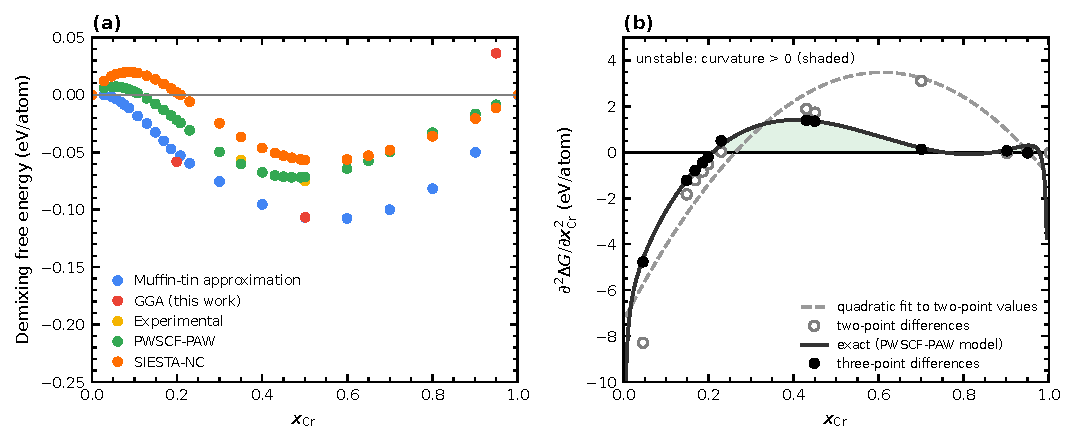
\includegraphics[width=\linewidth]{figures/fig1_free_energy.pdf}
\caption{(a) Demixing free energy $\Delta G_{\mathrm{demix}} = -\Delta G_{\mathrm{mix}}$ (Eq.~\ref{eqn:demix}) versus chromium composition $x_{\mathrm{Cr}}$: muffin-tin approximation, GGA (present VASP calculations), experiment, and the PWSCF--PAW and SIESTA--NC interaction models of Levesque \textit{et al.} \cite{levesque2011simple} at 298.15 K. (b) Curvature of the PWSCF--PAW demixing free energy. Solid line: exact analytic second derivative of the model. Filled circles: three-point second differences of its tabulated values on the non-uniform composition grid. Open circles: two-point second differences of the same values, with a quadratic least-squares fit (dashed). Shading marks positive demixing curvature, i.e., negative mixing curvature, which identifies spinodally unstable compositions.}
\label{fig:free_energy}
\end{figure}

Figure~\ref{fig:free_energy}b shows that the homogeneous alloy is unstable for $0.21 \lesssim x_{\mathrm{Cr}} \lesssim 0.75$ in the PWSCF--PAW model (with a second, narrow window at $0.87$--$0.98$); the SIESTA--NC model gives $0.25 \lesssim x_{\mathrm{Cr}} \lesssim 0.99$. Both windows contain the Fe--36Cr alloy in which spinodal decomposition was recently detected through TGS stiffening \cite{rae2026tgs}. Because the entropic term lowers the curvature in proportion to $T$, these windows narrow at the higher temperatures used for aging. Within them, elastic and acoustic properties cannot be interpreted assuming a homogeneous solid solution. Instead, any observable elastic response must be understood as emerging from a system that is intrinsically driven toward compositional modulation, providing the foundation for linking free-energy curvature to stiffness evolution and ultimately to ultrasonic observables.

\subsection{Elastic stiffening and elastodynamic mapping to Rayleigh SAW observables}

% --- FIGURE: elasticity + elastodynamics ---
\begin{figure}[!h]
\centering
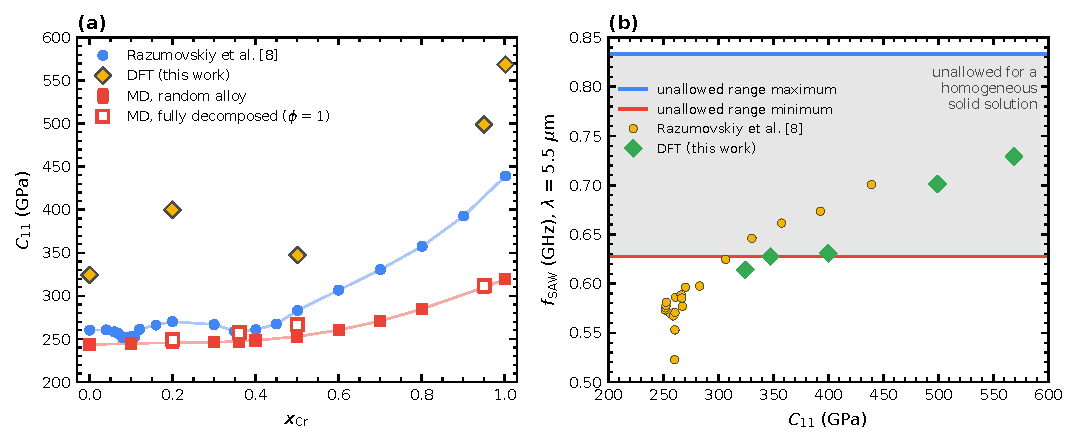
\includegraphics[width=\linewidth]{figures/fig2_elastic_mapping.pdf}
\caption{(a) $C_{11}$ of homogeneous \textit{bcc} Fe$_{1-x}$Cr$_x$: literature calculations of Razumovskiy \textit{et al.} \cite{razumovskiy2011first} (blue circles; reconstructed from digitized $C'$, $C_{44}$, and $B$) and present DFT calculations on 40-atom SQS (yellow diamonds). Red squares: MD (EAM) random alloys (mean $\pm$ standard deviation of ten alloys at the DFT compositions and three elsewhere; Sec.~\ref{sec:md}). Open red squares: fully decomposed MD structures ($\phi=1$), from Ref.~\cite{al2023detecting} at 50/50 and from the present $25^3$-cell calculations at $x_{\mathrm{Cr}}=0.20$, 0.36, and 0.95. (b) Rayleigh SAW frequency versus $C_{11}$ for the literature (yellow) and DFT (green) data, at $\lambda=5.5\,\mu$m. The shaded region is the elastodynamically unallowed range of Ref.~\cite{al2023detecting} (Fig.~9 therein), between the maximum pseudo-SAW frequency (0.627 GHz) and the bulk-wave frequency (0.833 GHz) calculated for pristine 304-type CASS.}
\label{fig:elastic_elastodynamics}
\end{figure}

To connect thermodynamic instability to experimentally measurable quantities, we compute the cubic elastic tensor across $x_{\mathrm{Cr}}$ and propagate these elastic inputs through the surface boundary-value problem of Sec.~2.1. Although $f_{\mathrm{SAW}}$ depends on the full tensor through $B$ and $G$, we use the longitudinal stiffness $C_{11}$ as a compact index of composition-dependent stiffening (Fig.~\ref{fig:elastic_elastodynamics}a). The blue points are literature calculations by Razumovskiy \textit{et al.} \cite{razumovskiy2011first}, the yellow diamonds are ours, and the red squares are MD (EAM) random alloys computed here with the procedure of our earlier study \cite{al2023detecting}; the open squares are the corresponding fully decomposed structures, which are stiffer than the random alloy at every composition, most strongly at intermediate compositions (e.g., 257.4 versus 247.3 GPa at $x_{\mathrm{Cr}}=0.36$). The present DFT tensors are systematically stiffer than the reference data (e.g., $C_{11}=324$ versus 260 GPa for \textit{bcc} Fe) and correspondingly predict higher frequencies. Possible contributors include the $\Gamma$-point-only $k$-point sampling, the finite SQS size, and the magnetic configuration. We therefore interpret relative trends rather than absolute frequencies.

As shown in Fig.~\ref{fig:elastic_elastodynamics}, $C_{11}$ depends systematically on chromium concentration (non-monotonically in the literature and DFT data), producing corresponding shifts in the Rayleigh SAW frequency. For a homogeneous solid solution, each composition corresponds to a single tensor and hence a single $f_{\mathrm{SAW}}$. In our earlier study, elastodynamic calculations for pristine CASS over randomly sampled grain orientations defined an ``unallowed'' frequency range, above the highest (pseudo-)SAW frequency and below the bulk-wave frequency, in which no surface mode of the pristine material exists; (P)SAW peaks observed there after aging were attributed to stiffened $\delta$-ferrite \cite{al2023detecting}. Figure~\ref{fig:elastic_elastodynamics}b places the homogeneous Fe--Cr frequencies relative to that range: alloys up to $x_{\mathrm{Cr}}\approx0.6$ lie below it, and only Cr-rich compositions approach or enter it. Frequencies in this range therefore indicate stiffness beyond that of a homogeneous solid solution of $\delta$-ferrite or Fe--36Cr composition, consistent with the stiffer Cr-rich $\alpha'$ regions formed by spinodal decomposition (Fig.~\ref{fig:fsaw_combined}a). Within the spinodally unstable composition window, elastic stiffening therefore translates into measurable acoustic signatures, enabling stiffness changes to be inferred non-destructively.

\subsection{Separating composition trends from spinodal conversion trends}

While elastic constants vary with chromium concentration even in a homogeneous solid solution, spinodal decomposition introduces an additional, time-dependent microstructural evolution. To disentangle these effects, it is necessary to distinguish changes driven purely by composition from those arising from the progression of phase separation. We therefore report two complementary relationships that isolate these contributions within a unified elastodynamic framework.

% --- FIGURE: fSAW vs xCr and vs phi ---
\begin{figure}[!h]
\centering
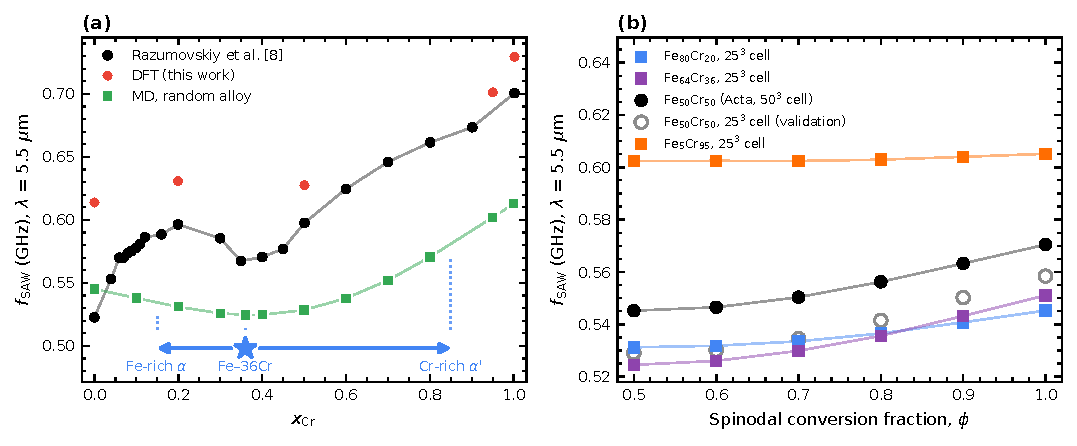
\includegraphics[width=\linewidth]{figures/fig3_fsaw.pdf}
\caption{(a) Rayleigh SAW frequency $f_{\mathrm{SAW}}$ versus chromium composition $x_{\mathrm{Cr}}$ ($\lambda=5.5\,\mu$m) for the literature (black), present DFT (red), and MD random-alloy (green) data of Fig.~\ref{fig:elastic_elastodynamics}. Below the data, the star marks Fe--36Cr \cite{rae2026tgs} and the arrows indicate schematically the partitioning toward Fe-rich $\alpha$ and Cr-rich $\alpha'$ during spinodal decomposition; dotted lines rise from each composition toward the data. Arrow endpoints are illustrative, not measured phase compositions. (b) $f_{\mathrm{SAW}}$ versus spinodal conversion fraction $\phi$ from the MD (EAM) decomposition simulations (Sec.~\ref{sec:md}): equiatomic Fe$_{50}$Cr$_{50}$ from Ref.~\cite{al2023detecting} (black, $50^3$ cell, fixed density 7535 kg m$^{-3}$), and Fe$_{80}$Cr$_{20}$, Fe$_{64}$Cr$_{36}$, and Fe$_{5}$Cr$_{95}$ from the present $25^3$-cell calculations (squares); open circles repeat Fe$_{50}$Cr$_{50}$ in the $25^3$ cell as a check. $\phi=0.5$ is the random alloy and $\phi=1$ the fully separated structure.}
\label{fig:fsaw_combined}
\end{figure}

Figure~\ref{fig:fsaw_combined}a shows how chromium partitioning produces stiffening. The Fe--36Cr composition lies near a local minimum of the homogeneous $f_{\mathrm{SAW}}(x_{\mathrm{Cr}})$ curve. Spinodal decomposition moves material toward Fe-rich $\alpha$ and Cr-rich $\alpha'$ compositions (arrows); in both directions the homogeneous-alloy frequency increases. The DFT set, with only five compositions, is consistent with this non-monotonic dependence but cannot resolve the minimum. The MD random alloys, an independent classical model, also show a frequency minimum, at $x_{\mathrm{Cr}}\approx0.36$--0.40, i.e.\ at the Fe--36Cr composition, even though their $C_{11}$ increases monotonically (Fig.~\ref{fig:elastic_elastodynamics}a): the minimum comes from the shear moduli, which control the Rayleigh velocity ($C_{44}$ decreases from 116 GPa for Fe to 106 GPa at $x_{\mathrm{Cr}}=0.5$). $C_{11}$ is therefore a convenient index of stiffening, but the SAW response is governed by shear stiffness. Figure~\ref{fig:fsaw_combined}a describes the properties of the constituents; the effective response of the two-phase microstructure additionally depends on phase fractions and on the domain size relative to the SAW wavelength.

Figure~\ref{fig:fsaw_combined}b isolates the effect of decomposition at fixed overall composition (Fe$_{50}$Cr$_{50}$). In the MD (EAM) simulations, $f_{\mathrm{SAW}}$ increases monotonically from 0.545 GHz for the random alloy ($\phi=0.5$) to 0.570 GHz for the fully separated structure ($\phi=1$), an increase of about 4.6\% under the fixed-density assumption. The empirical-potential and first-principles results therefore agree in sign. Repeating the decomposition at other compositions (Sec.~\ref{sec:md}) gives frequency increases between the random and fully separated states of 2.6\%, 5.1\%, 5.5\%, and 0.5\% for $x_{\mathrm{Cr}}=0.20$, 0.36, 0.50, and 0.95, respectively. Stiffening on decomposition is therefore largest within the spinodally unstable window of Fig.~\ref{fig:free_energy}b, including the Fe--36Cr composition, and nearly vanishes for the dilute Cr-rich alloy. The fully separated state is an idealized limit, so these values bound the stiffening from above. At 50/50, the small-cell series lies about 2\% below the original series in absolute frequency because the original moduli used a different isotropic average; the relative changes agree to within one percentage point. Together, $f_{\mathrm{SAW}}(x_{\mathrm{Cr}})$ captures the baseline elastic response of a homogeneous alloy, and $f_{\mathrm{SAW}}(\phi)$ reflects the additional stiffening associated with progressive spinodal conversion. This separation enables experimental SAW measurements to be interpreted in terms of both composition and decomposition state, providing a pathway to distinguish early-stage spinodal evolution from equilibrium compositional effects.


\section{Discussion}

Taken together, the results establish a closed thermodynamics-to-observable pathway for interpreting picosecond ultrasonic measurements in $\delta$--ferrite–containing stainless steels. The free-energy curvature criterion identifies the composition window in which the homogeneous solid solution is intrinsically unstable, defining the regime where elastic and acoustic properties must reflect ongoing or incipient spinodal decomposition rather than equilibrium alloy behavior.

Within this thermodynamically unstable regime, first-principles elasticity reveals systematic stiffening trends that are propagated through elastodynamic constraints into Rayleigh SAW frequency shifts. The direct mapping between elastic constants and SAW observables provides a quantitative basis for interpreting peak shifts and splitting as signatures of stiffness evolution, rather than purely phenomenological indicators.

Crucially, separating the solid-solution trend $f_{\mathrm{SAW}}(x_{\mathrm{Cr}})$ from the spinodal conversion trend $f_{\mathrm{SAW}}(\phi)$ resolves a key ambiguity in experimental interpretation. While composition alone can shift SAW frequencies, progressive spinodal decomposition introduces additional stiffening that cannot be captured by composition-dependent elasticity alone. The combined framework therefore enables SAW peak splitting to be interpreted as a mechanistically grounded indicator of microstructural evolution toward embrittlement, rather than as a purely compositional effect.

This separation clarifies why SAW peak splitting emerges as a robust, non-destructive diagnostic of spinodal decomposition in CASS and related alloys, and suggests a general strategy for extending ultrasonic embrittlement detection to other phase-separating structural materials.


\section{Conclusions}
We presented a compact thermodynamics-to-elastodynamics workflow for bcc Fe--Cr $\delta$--ferrite that links demixing free-energy curvature, first-principles elastic constants, and Rayleigh SAW observables. Free-energy curvature provides a direct stability criterion that identifies spinodally unstable composition windows. DFT-derived cubic elasticity quantifies composition-dependent stiffening trends and supplies inputs for elastodynamic prediction. Combining these elements yields experimentally actionable relationships for interpreting picosecond ultrasonics across both composition and decomposition-state variables.

\section*{Data Availability}
The tabulated data, the atomistic and first-principles simulation inputs and outputs, and the scripts that generate all figures will be made publicly available at \url{https://github.com/saleemaldajani/elastopya}, with an archived DOI.


\bibliographystyle{elsarticle-num}
\bibliography{references}


\newpage
\clearpage

\section*{Supplementary Material}

\setcounter{figure}{0}
\renewcommand{\thefigure}{S\arabic{figure}}

\subsection*{S1. Thermal transport estimates}

Thermal properties in Fig.~\ref{fig5} are estimated with the Debye model, and a lower limit for the thermal conductivity is obtained at high temperature \cite{clarke2003materialsselection,clarke2003materialsdesign}:
\begin{eqnarray}
    \kappa &=& \frac{1}{3} C_v v_m \Lambda \\
    \kappa_{min} \rightarrow k_B v_m \Lambda \rightarrow k_B v_m \Lambda_{min} &=& A k_B \left(\frac{N_A m}{M}\right)^{\frac{2}{3}} \rho^{\frac{1}{6}} E^{\frac{1}{2}} \\
    \Theta_D &=& \frac{2\hbar v_m}{a_0 k_B} \rightarrow B_D \frac{\hbar}{k_B} \left(\frac{N_A m}{M}\right)^{\frac{1}{3}} \frac{E^{\frac{1}{2}} }{\rho^{\frac{1}{6}}}
\end{eqnarray}
where $\kappa$ is thermal conductivity, $\Theta_D$ is the Debye temperature, $C_v$ is the heat capacity at constant volume, $v_m$ is the average acoustic velocity, $\Lambda$ is the phonon mean free path, $m$ is the number of atoms, $M$ is the mass, $\rho$ is the density, and $E$ is Young's modulus. The constants $A$ and $B_D$ arise from approximating $v_m$ as proportional to $\sqrt{E/\rho}$; we use $A=0.87$ following Clarke \cite{clarke2003materialsselection}. A temperature-dependent alternative is the Cahill--Watson--Pohl model, $\kappa_{min} (T) = (\frac{\pi}{6})^{\frac{1}{3}} k_B n^{\frac{2}{3}} \sum_{i} v_i (\frac{T}{\Theta_i})^2 \int_{0}^{\Theta_i/T} \frac{x^3 e^x}{(e^x -1)^2}\,dx$ with $\Theta_i = v_i (\hbar/k_B) (6\pi^2n)^{\frac{1}{3}}$ \cite{cahill1992lower}.

\subsection*{S2. Additional figures}
The following figures are retained from the original draft for completeness and traceability.



\begin{figure}[!ht]
\centering
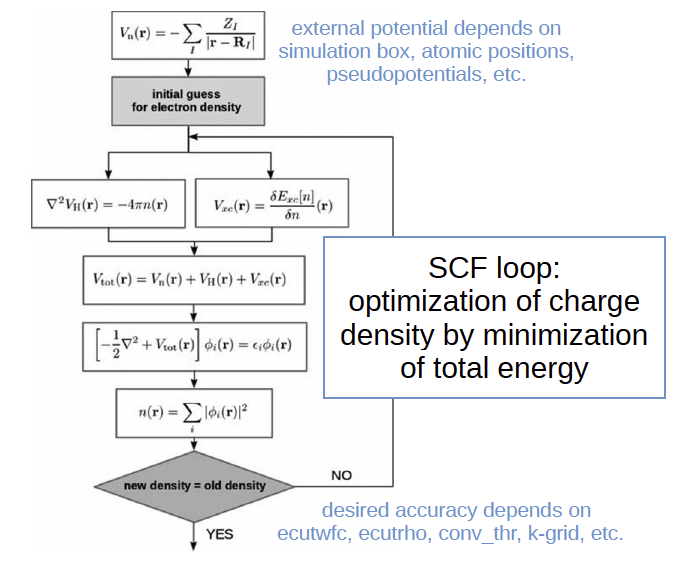
\includegraphics[width=0.85\textwidth]{figures/SCF.png}
\caption{Self-consistent field (SCF) loop schematic illustrating self-consistent electronic-structure workflow \cite{giustino2014materials}.}
\label{fig:SCF-loop}
\end{figure}


\begin{figure}[h!]
    \centering
    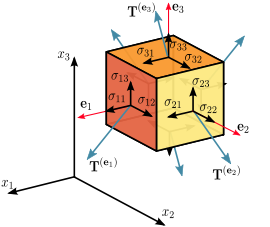
\includegraphics[width=0.6\textwidth]{Parts/Figures/Cij.png}
    \caption{Stress tensor visualization \cite{al2020non}.}
    \label{fig:seis-refl-tech}
\end{figure}

\begin{figure}[!ht]
	\centering
	\begin{subfigure}{0.9\textwidth}
         \centering
         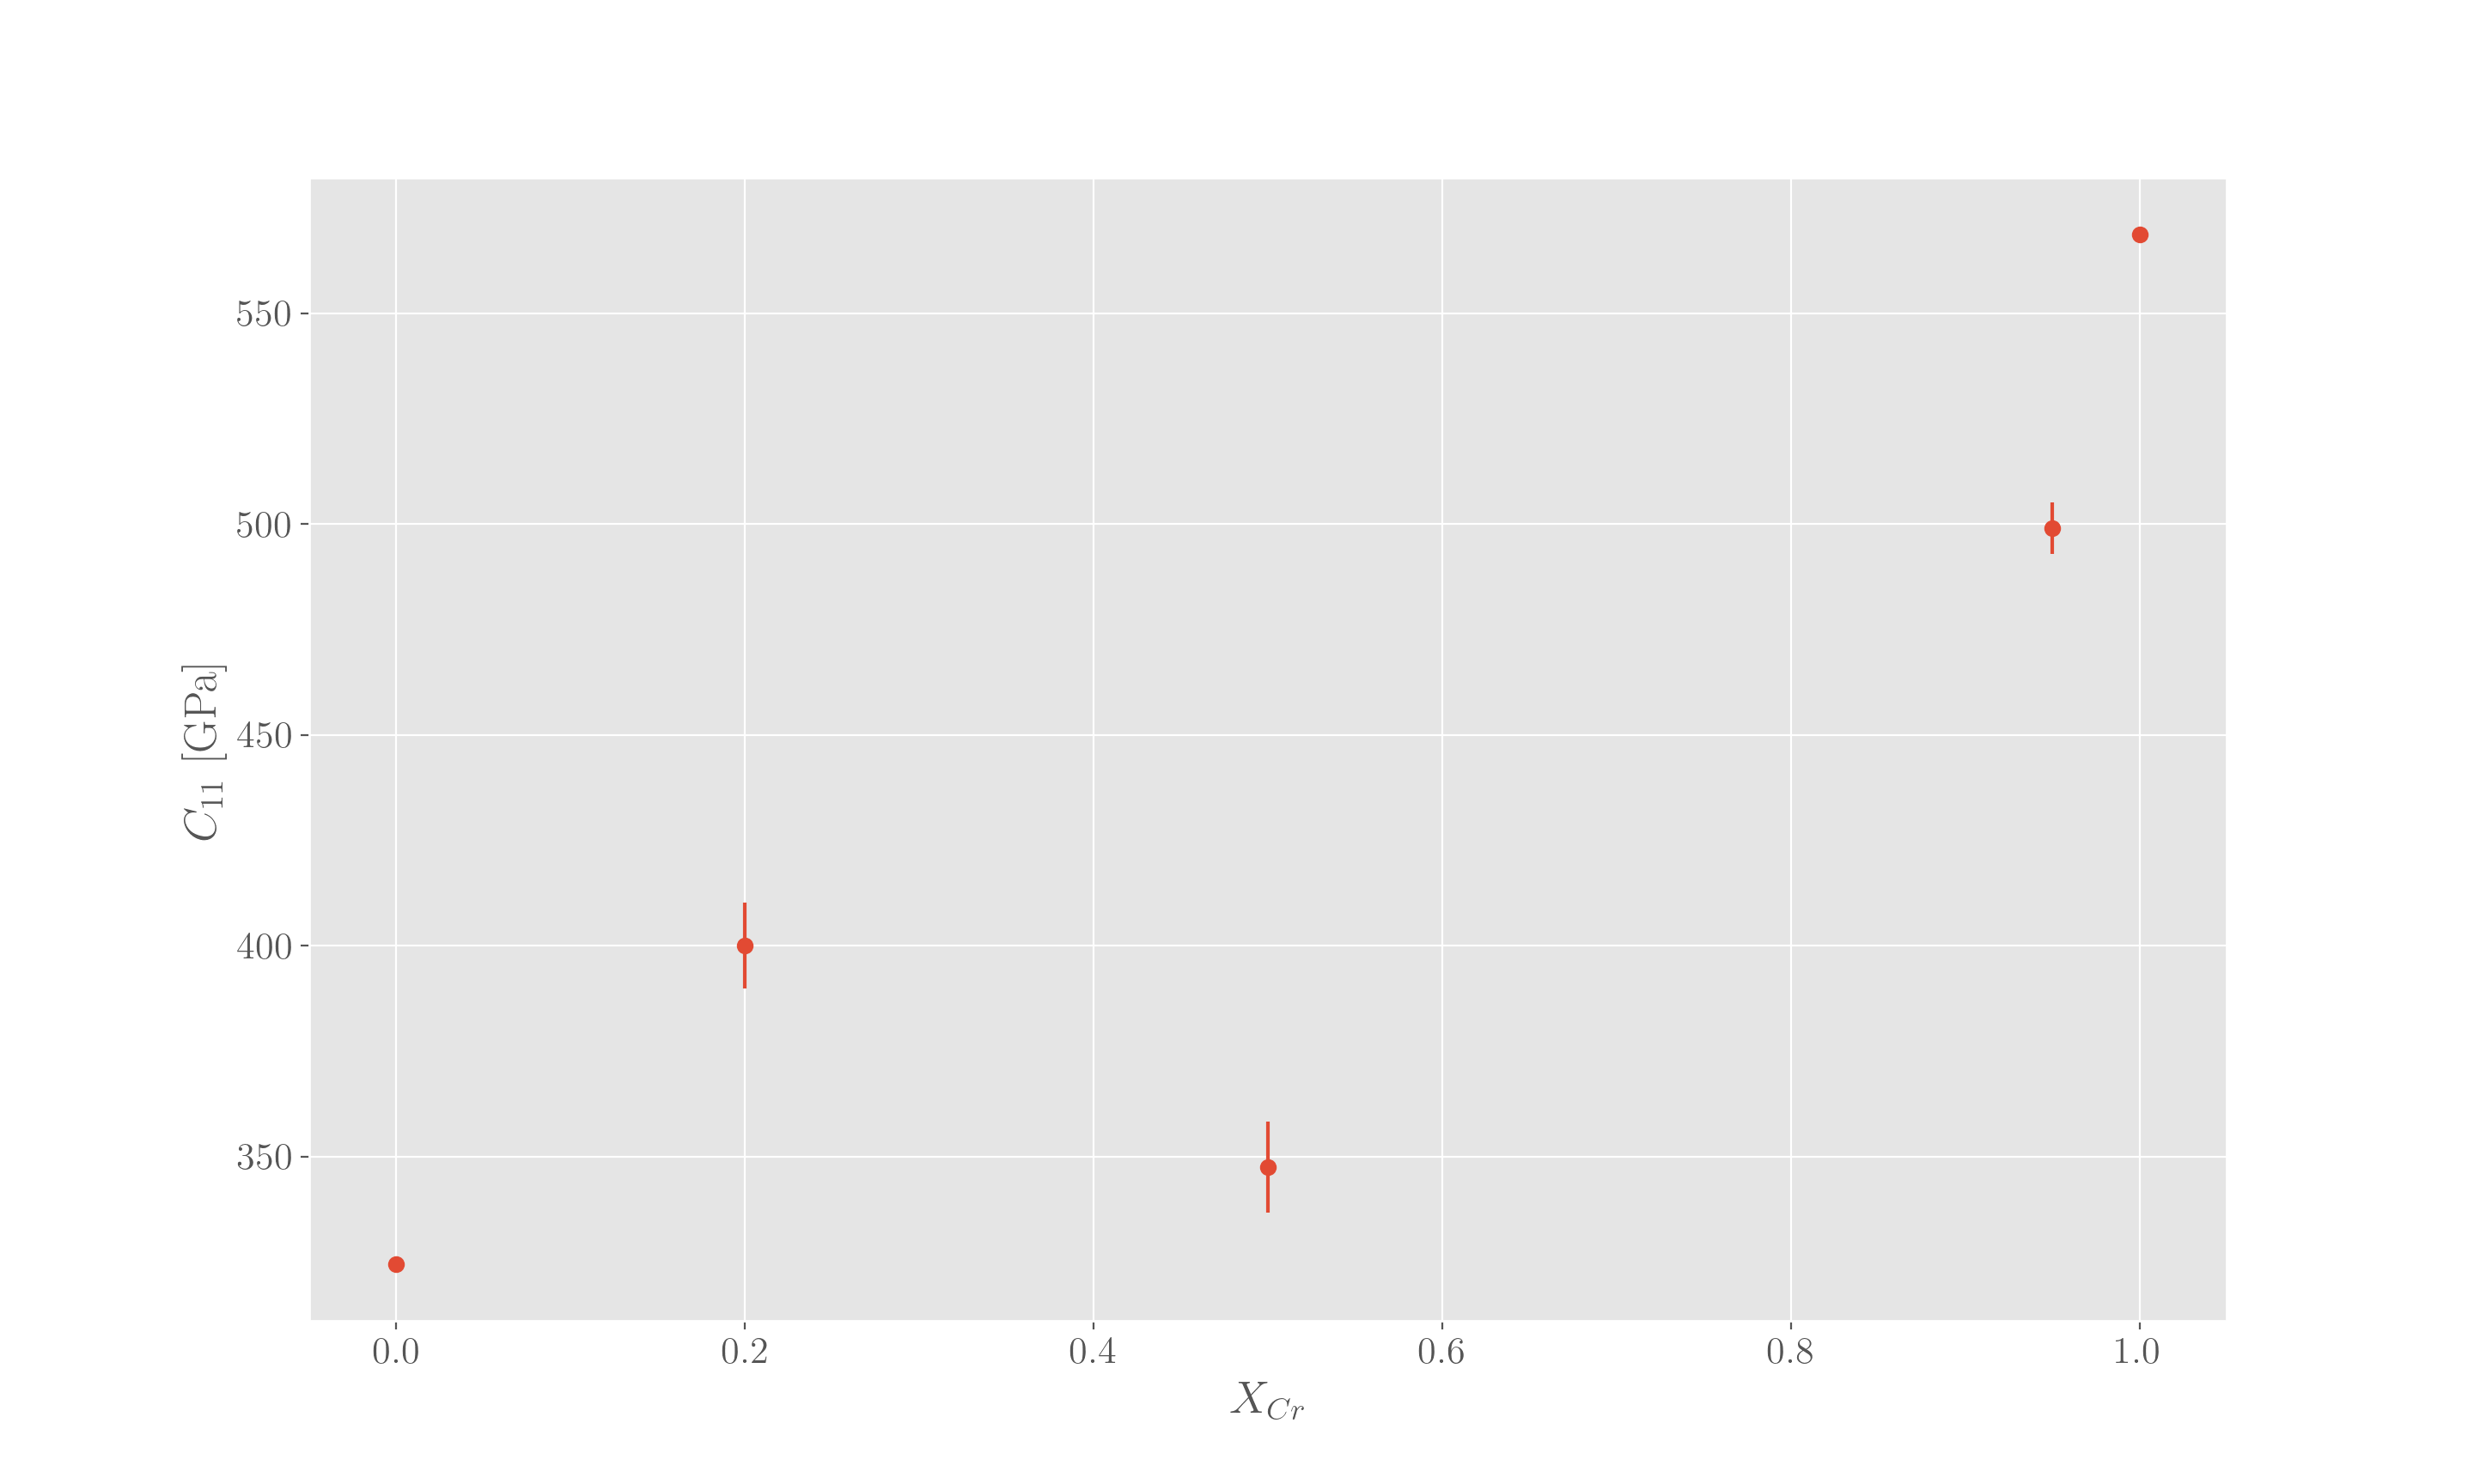
\includegraphics[width=\linewidth]{Parts/Figures/C11.png}
         \caption{Normal constant, \(C_{11}\), illustrating the longitudinal stiffness of bcc binary FeCr alloy as a function of chromium composition. This stiffness parameter is crucial for understanding the acoustic velocity and mechanical properties of the material.}
         \label{fig1a}
     \end{subfigure}
     \hfill
     \begin{subfigure}{0.45\textwidth}
         \centering
         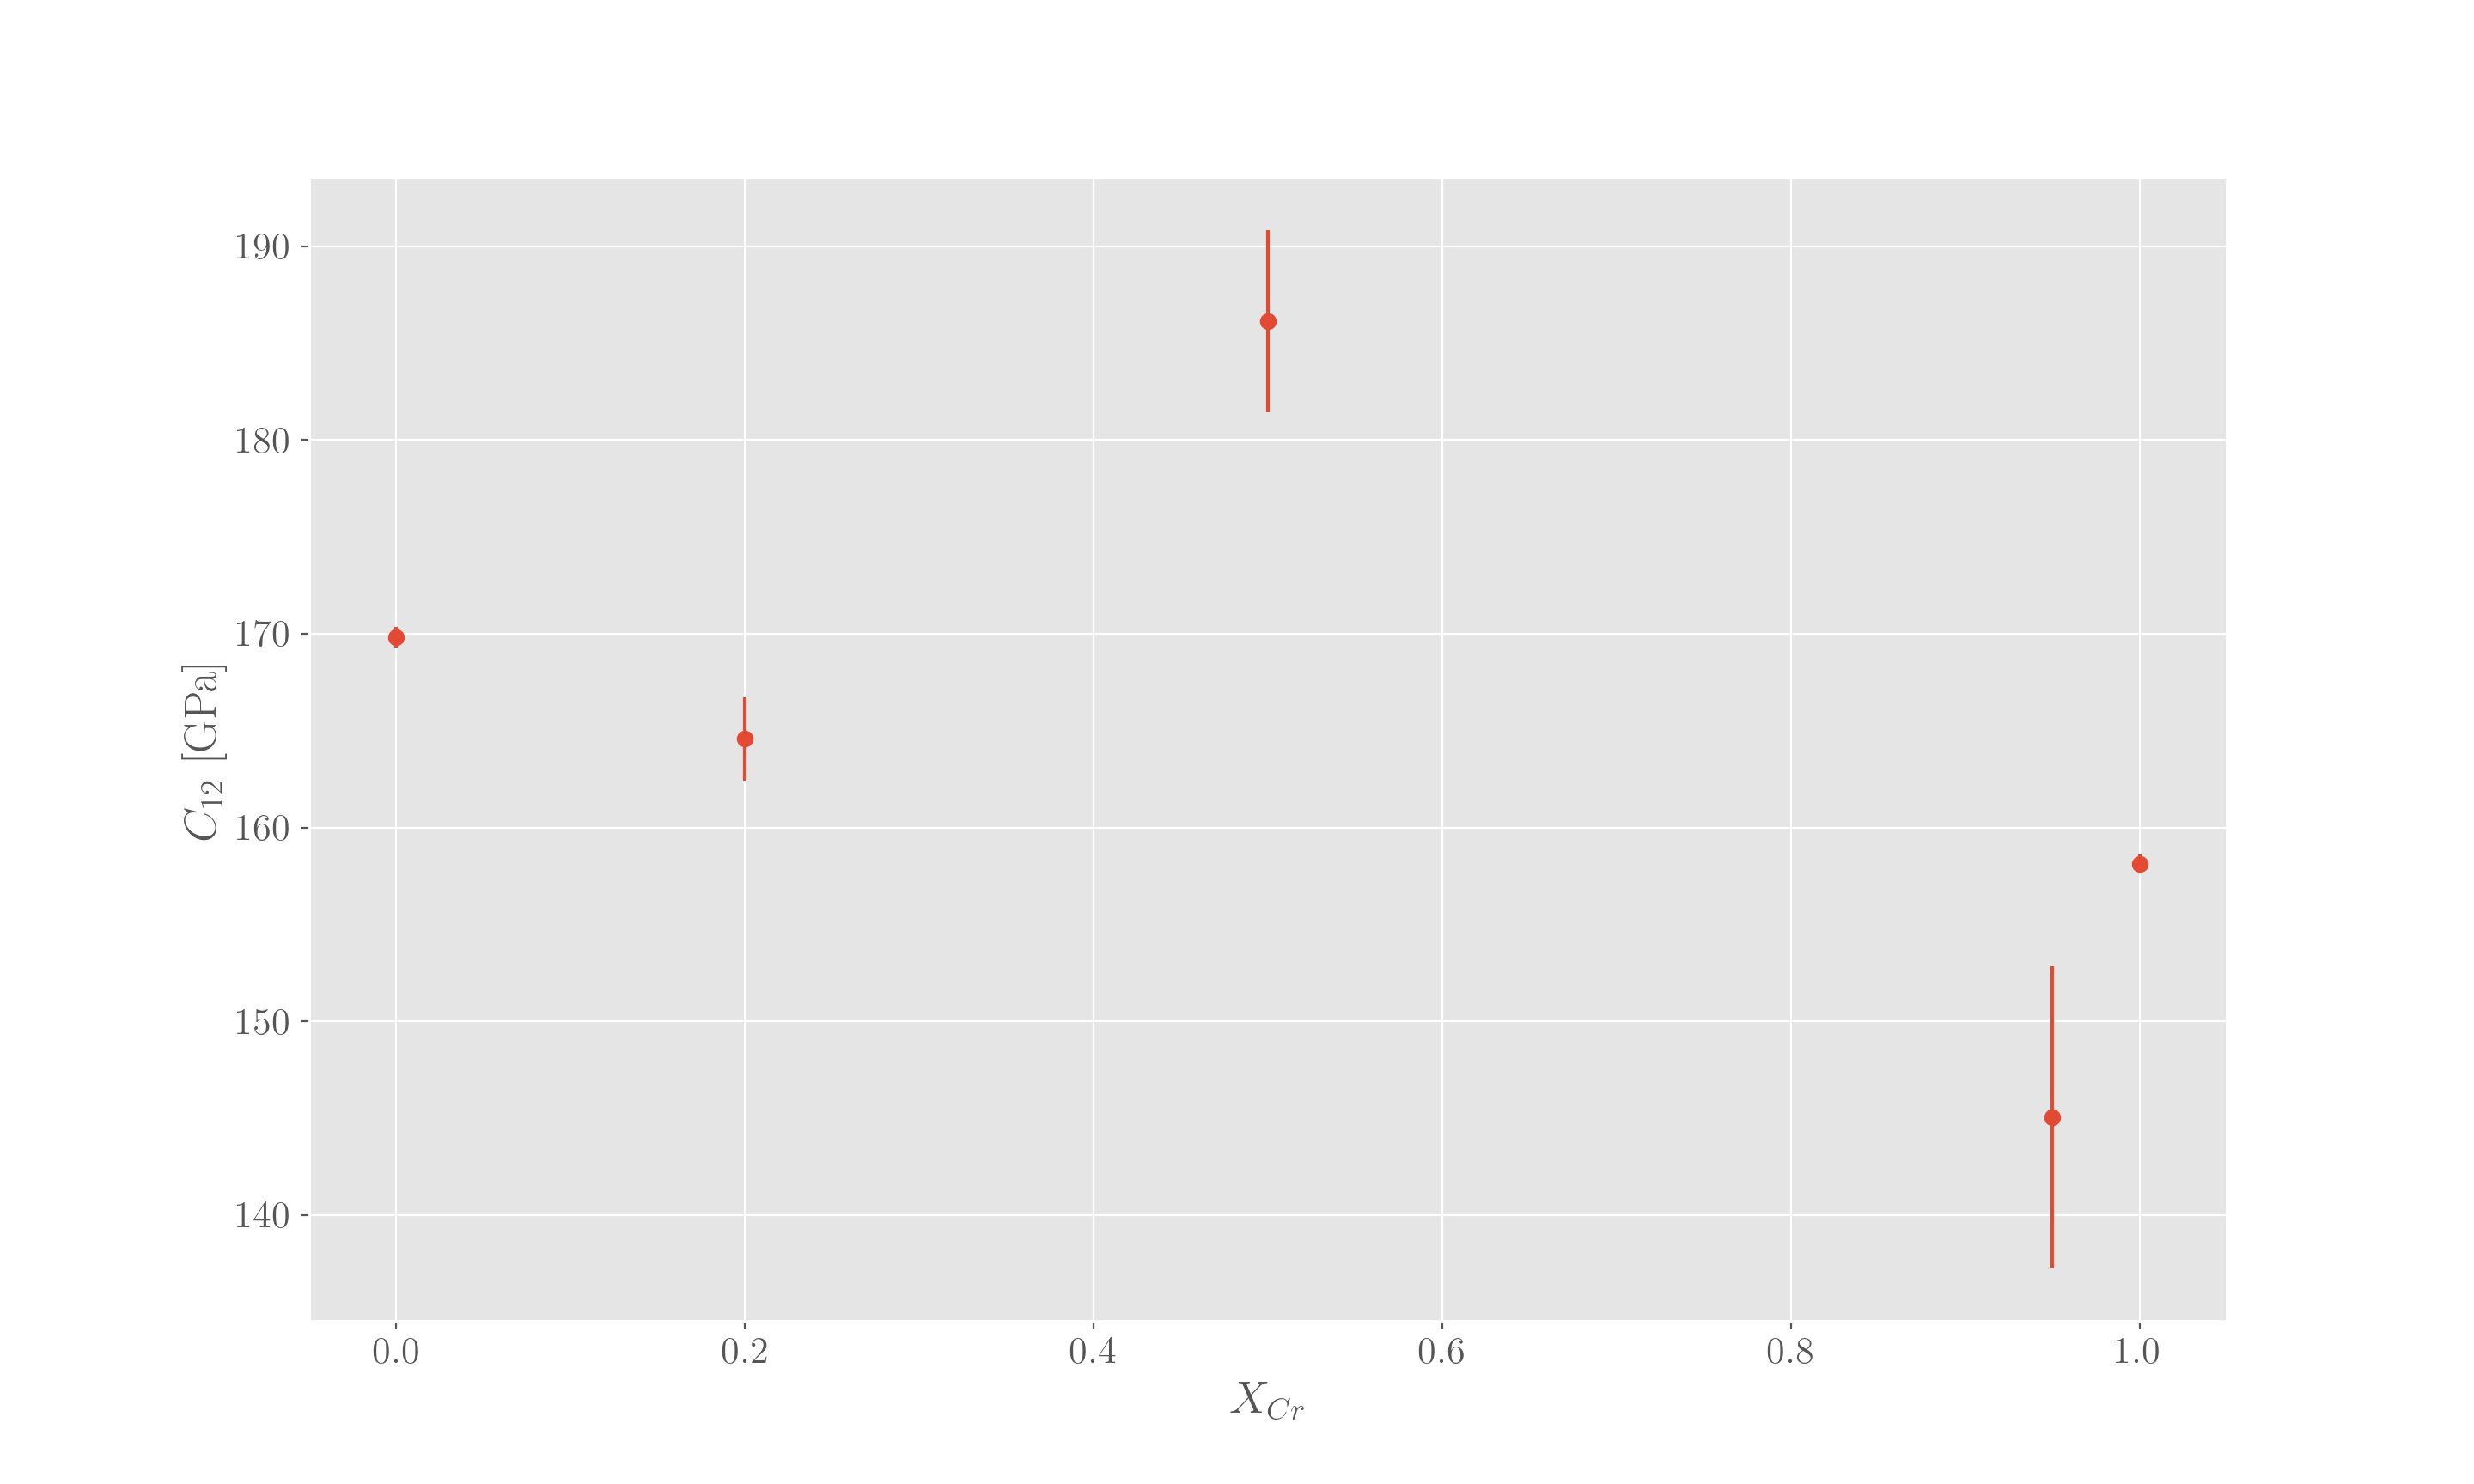
\includegraphics[width=\linewidth]{Parts/Figures/C12.png}
         \caption{The interplanar elastic constant \(C_{12}\), showing the coupling between axial and lateral strains, indicative of the alloy's resistance to shear along crystallographic planes.}
         \label{fig1b}
     \end{subfigure}
     \hfill
     \begin{subfigure}{0.45\textwidth}
         \centering
         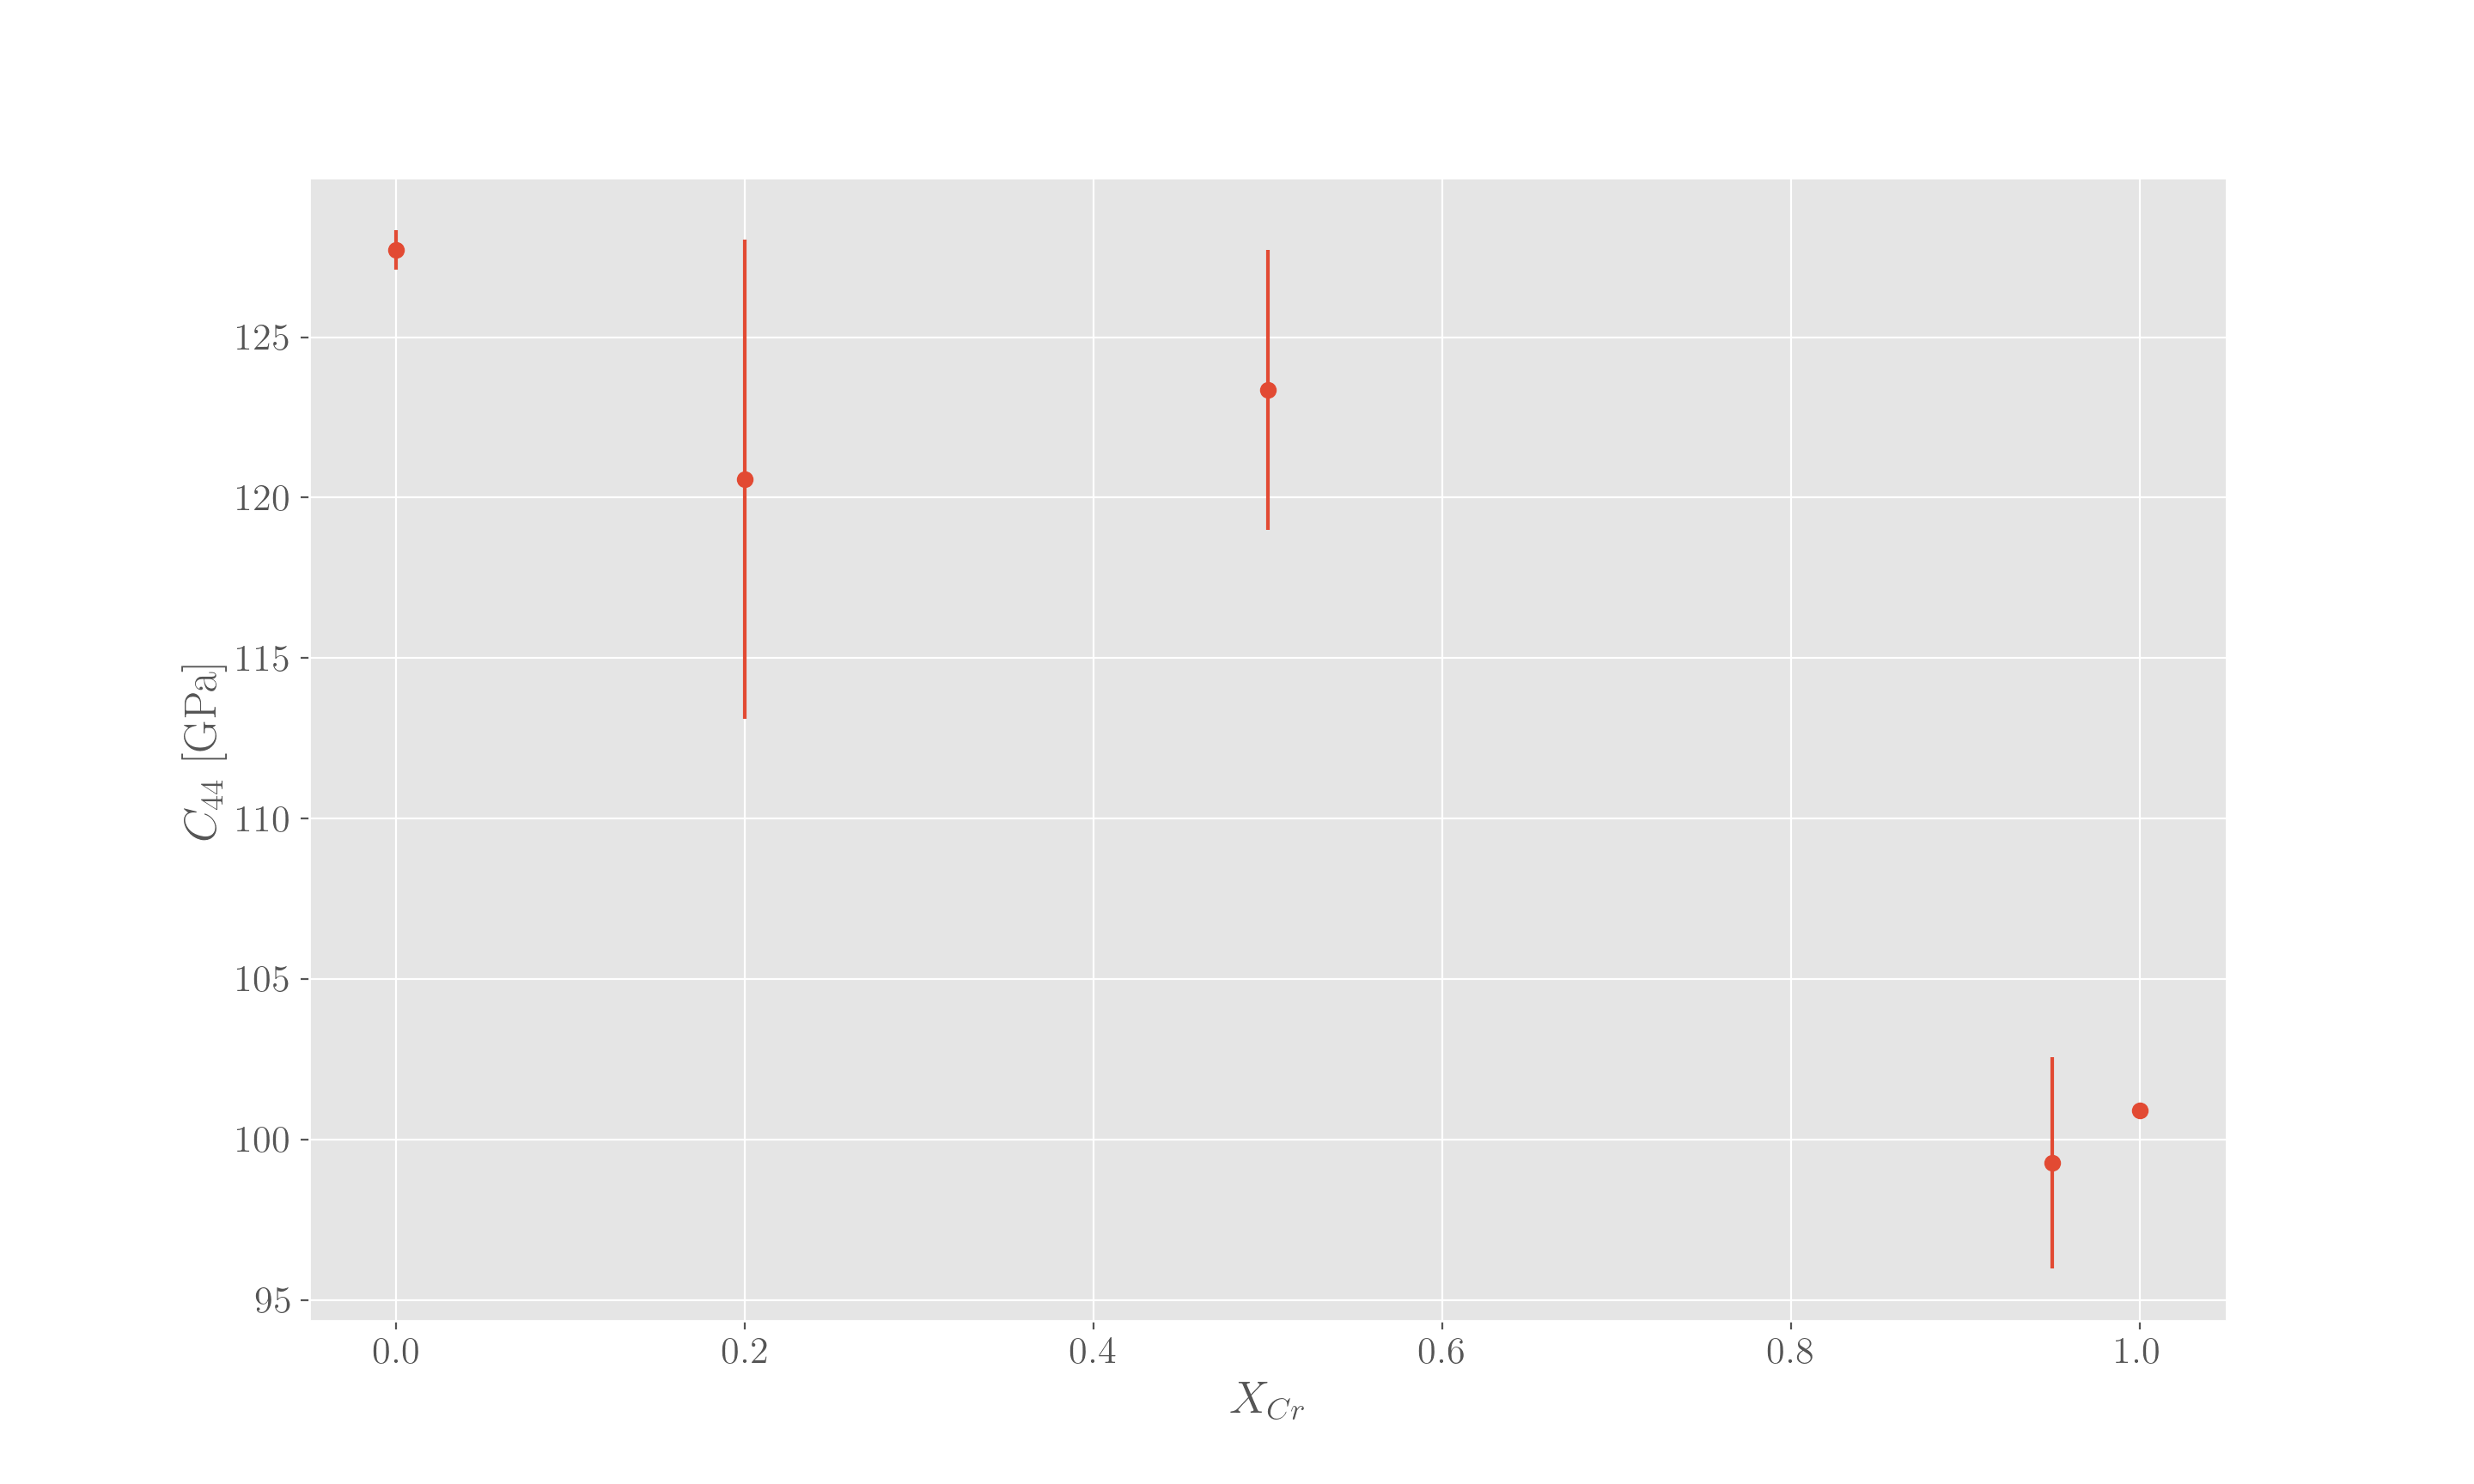
\includegraphics[width=\linewidth]{Parts/Figures/C44.png}
         \caption{Shear constant, \(C_{44}\), representing shear stiffness against deformation without volume change, critical for assessing material's resistance to applied shear stress.}
         \label{fig1c}
     \end{subfigure}
	\caption{Elastic constants of homogeneous bcc FeCr from the present DFT calculations (40-atom SQS) as a function of Cr composition. (a) Shows the longitudinal stiffness parameter \(C_{11}\), important for evaluating the material's response to compressive and tensile stresses. (b) Highlights \(C_{12}\), which is essential for understanding the coupling between different types of strain. (c) Details \(C_{44}\), crucial for evaluating the shear deformation behavior.}
	\label{fig1}
\end{figure}


\begin{figure}[!ht]
	\centering
	\begin{subfigure}{0.9\textwidth}
         \centering
         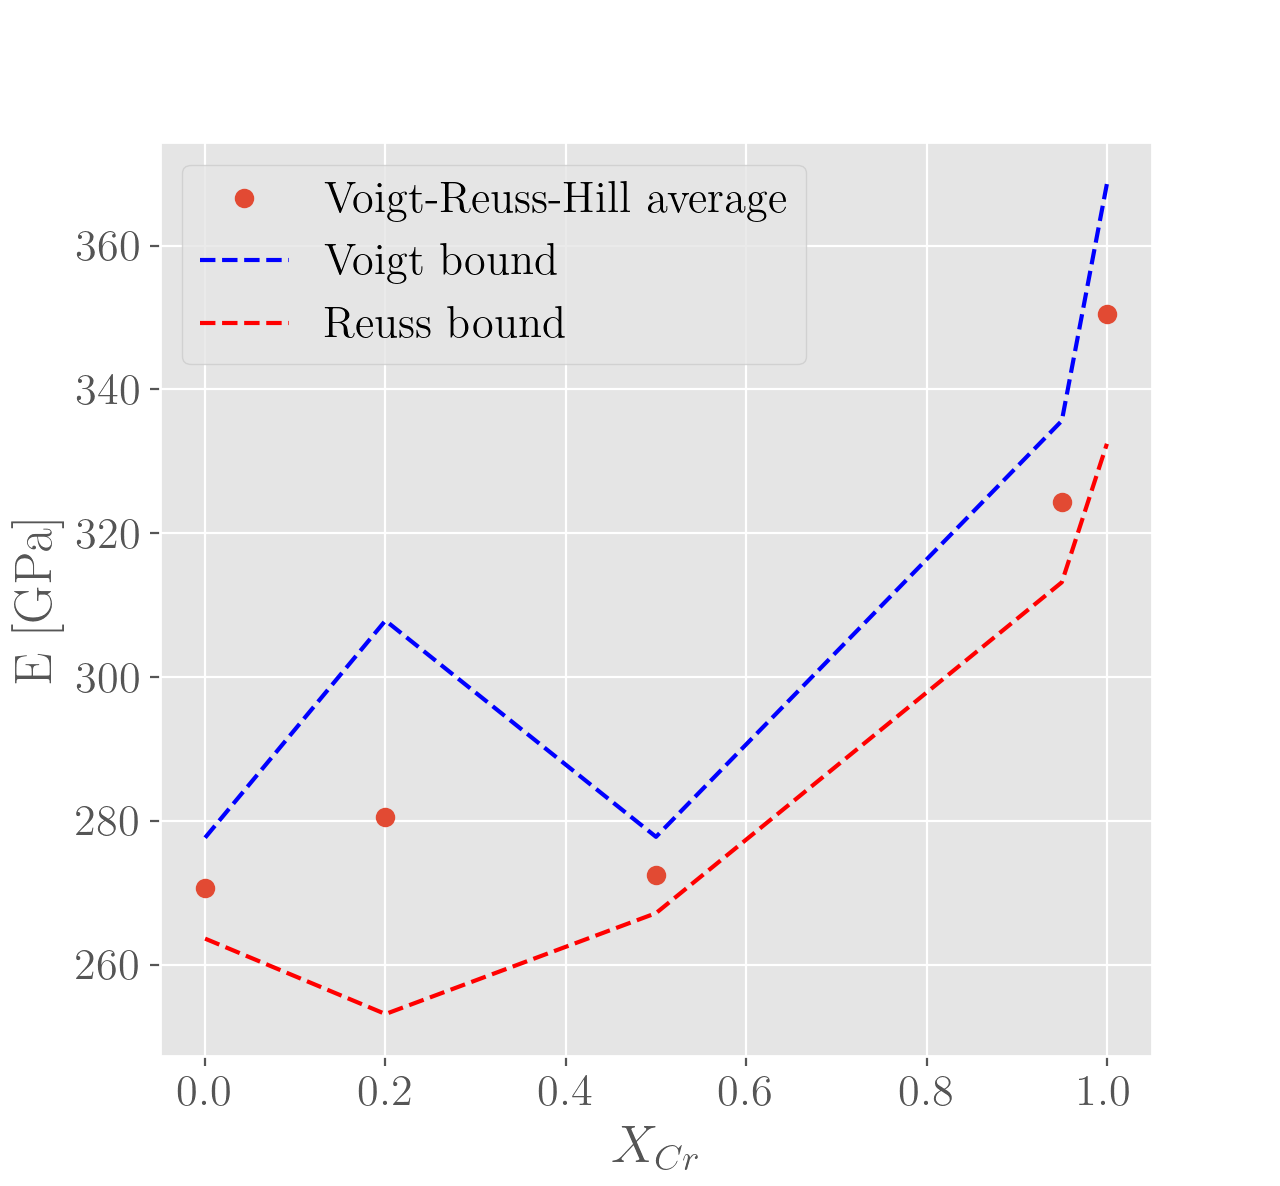
\includegraphics[width=0.9\linewidth]{Parts/Figures/E_VRH.png}
         \caption{Elastic (Young's) Modulus, \(E_{VRH}\), indicating the material's stiffness and its ability to resist deformation under tensile stress.}
         \label{fig2a}
     \end{subfigure}
     \hfill
     \begin{subfigure}{0.45\textwidth}
         \centering
         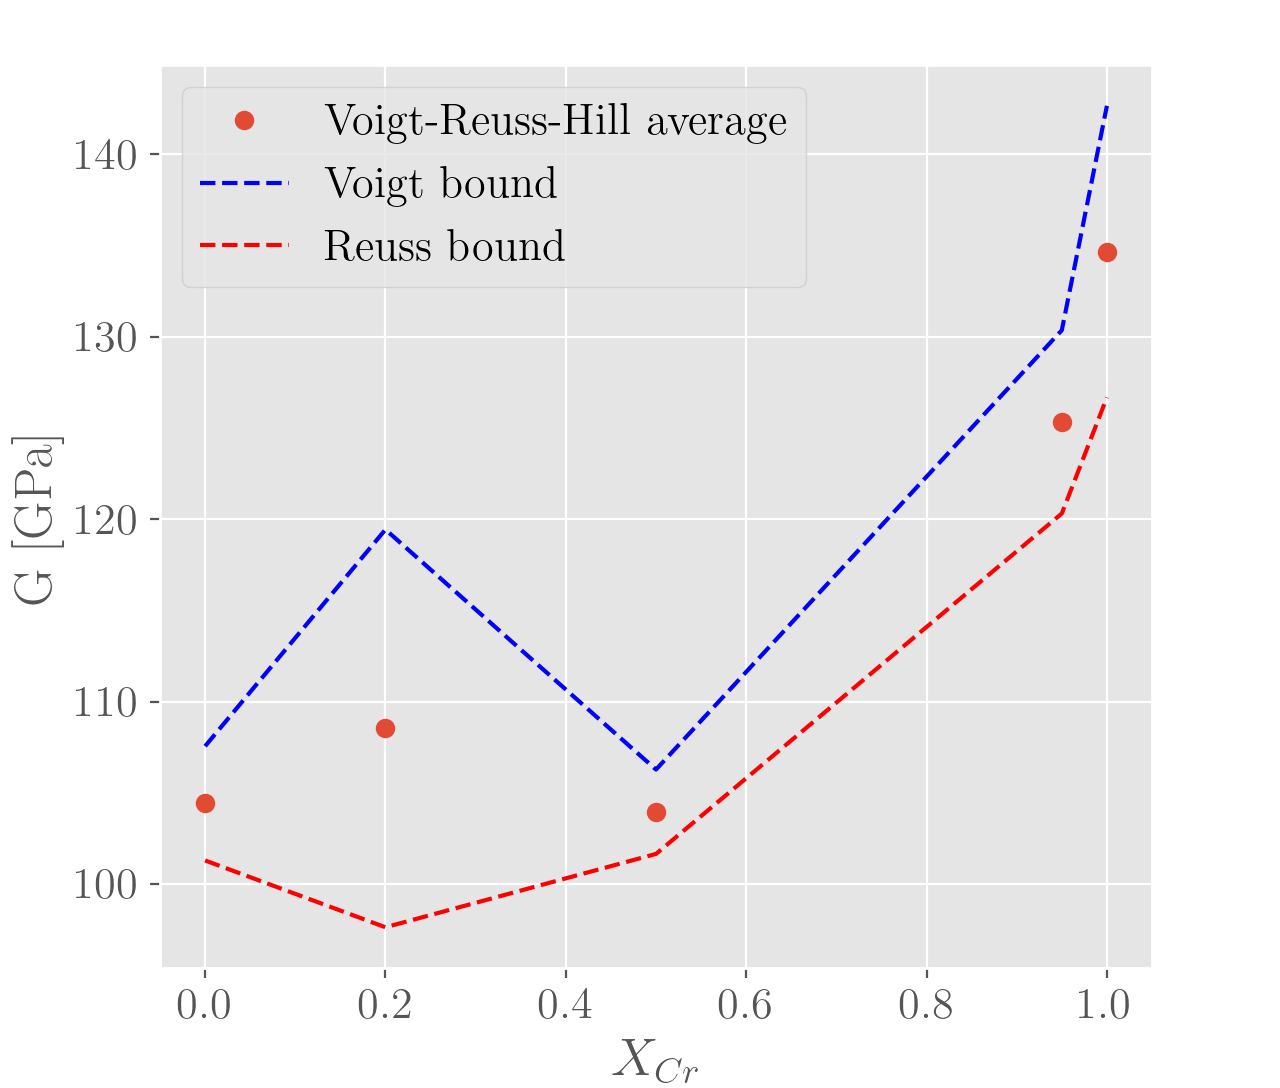
\includegraphics[width=\linewidth]{Parts/Figures/G_VRH.png}
         \caption{Shear modulus, \(G_{VRH}\), reflecting the material's ability to withstand shear deformation.}
         \label{fig2b}
     \end{subfigure}
     \hfill
     \begin{subfigure}{0.45\textwidth}
         \centering
         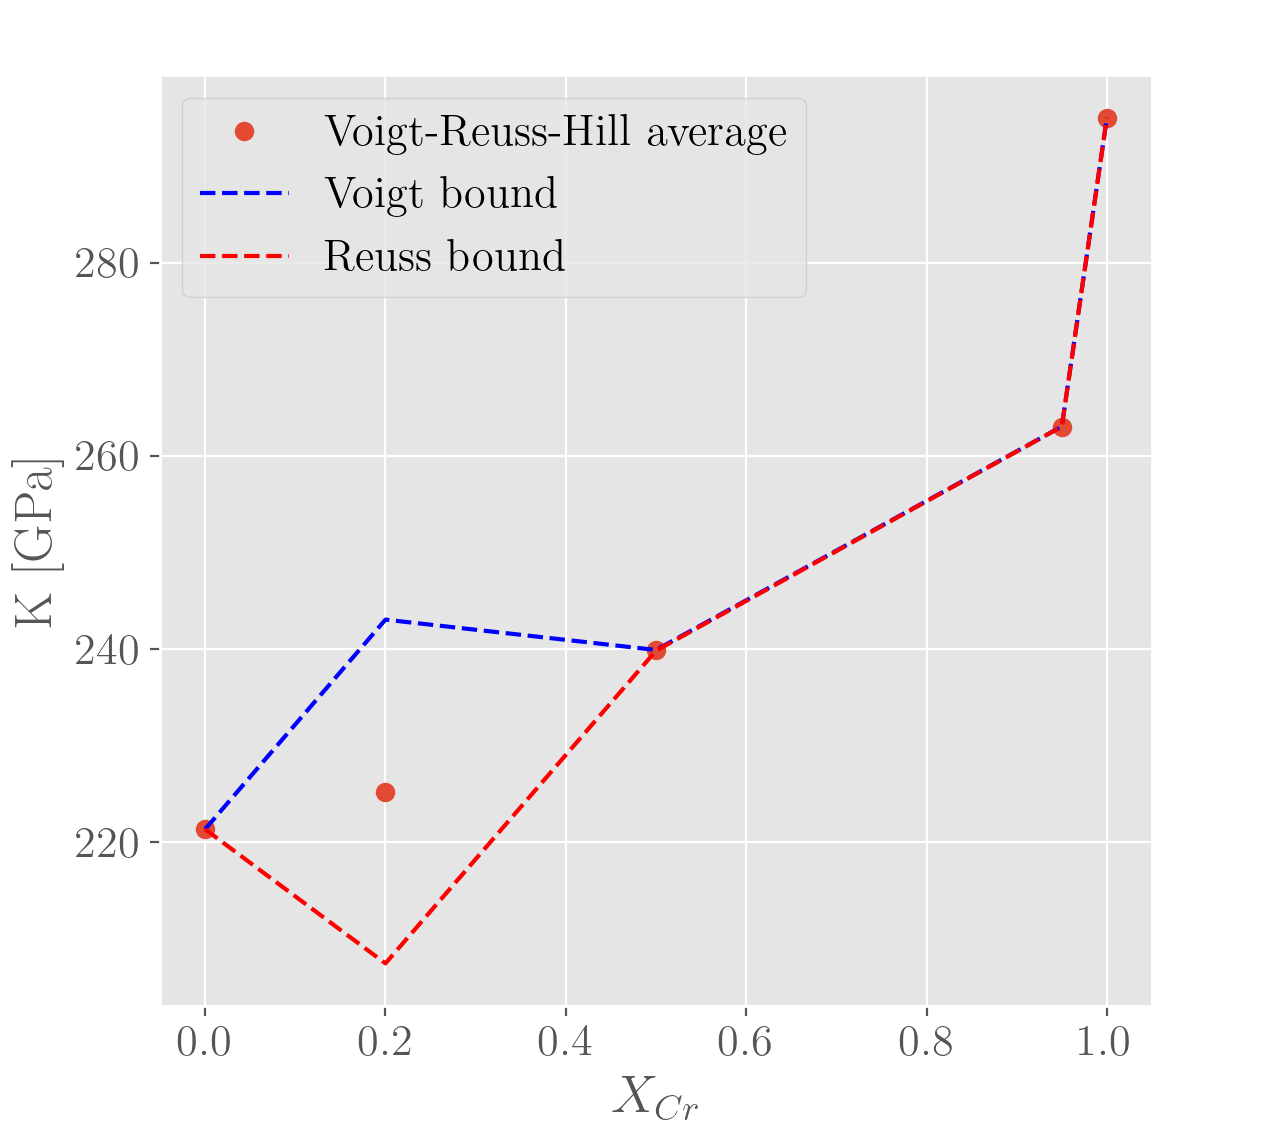
\includegraphics[width=\linewidth]{Parts/Figures/K_VRH.png}
         \caption{Bulk modulus, \(K_{VRH}\), which measures the material's resistance to uniform compression.}
         \label{fig2c}
     \end{subfigure}
	\caption{VRH elastic moduli of homogeneous bcc FeCr from the present DFT calculations as a function of Cr composition. (a) Elastic (Young's) Modulus demonstrates the material's overall stiffness. (b) Shear modulus is a measure of the alloy's rigidity against shear forces. (c) Bulk modulus assesses the material's compressibility under uniform pressure.}
	\label{fig2}
\end{figure}

\begin{sidewaysfigure}[!ht]
	\centering
	\begin{subfigure}{0.7\textwidth}
         \centering
         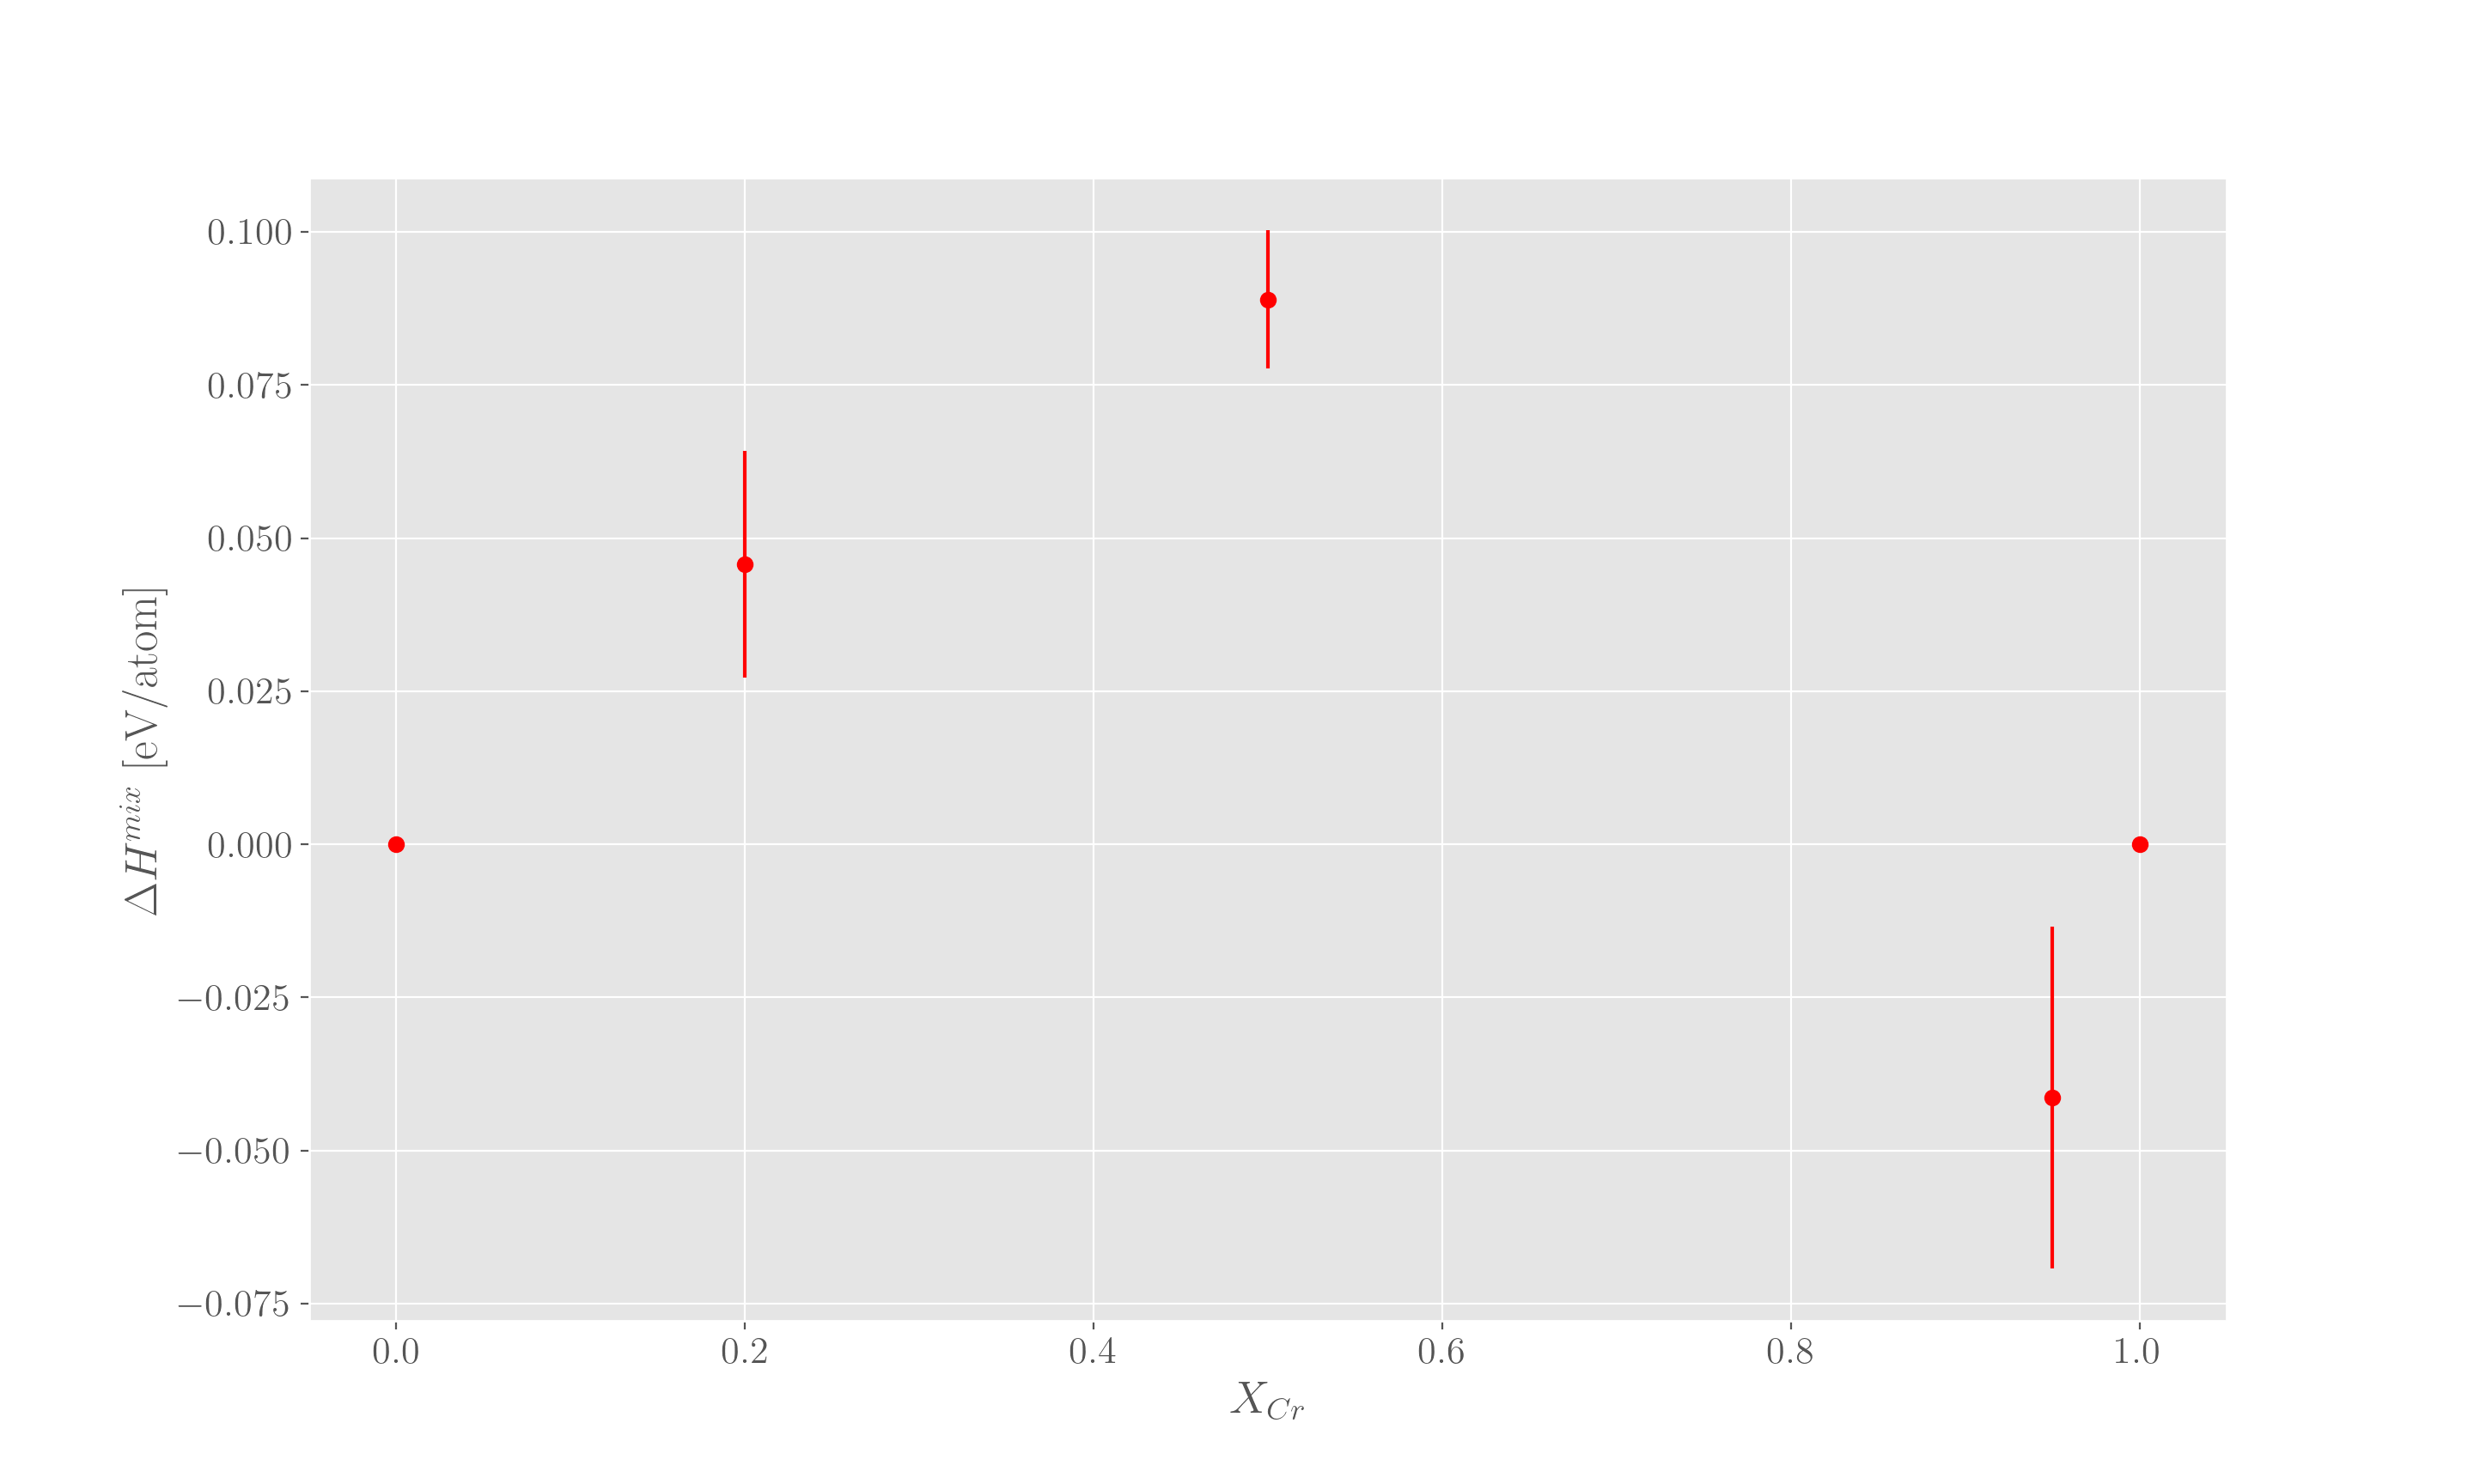
\includegraphics[width=\linewidth]{Parts/Figures/Hmix-vF.png}
         \caption{Enthalpy of mixing, showing the thermodynamic favorability of phase separation in bcc $\delta$-ferrite in cast austenitic stainless steels through spinodal decomposition.}
         \label{fig3a}
     \end{subfigure}
     \begin{subfigure}{0.3\textwidth}
         \centering
         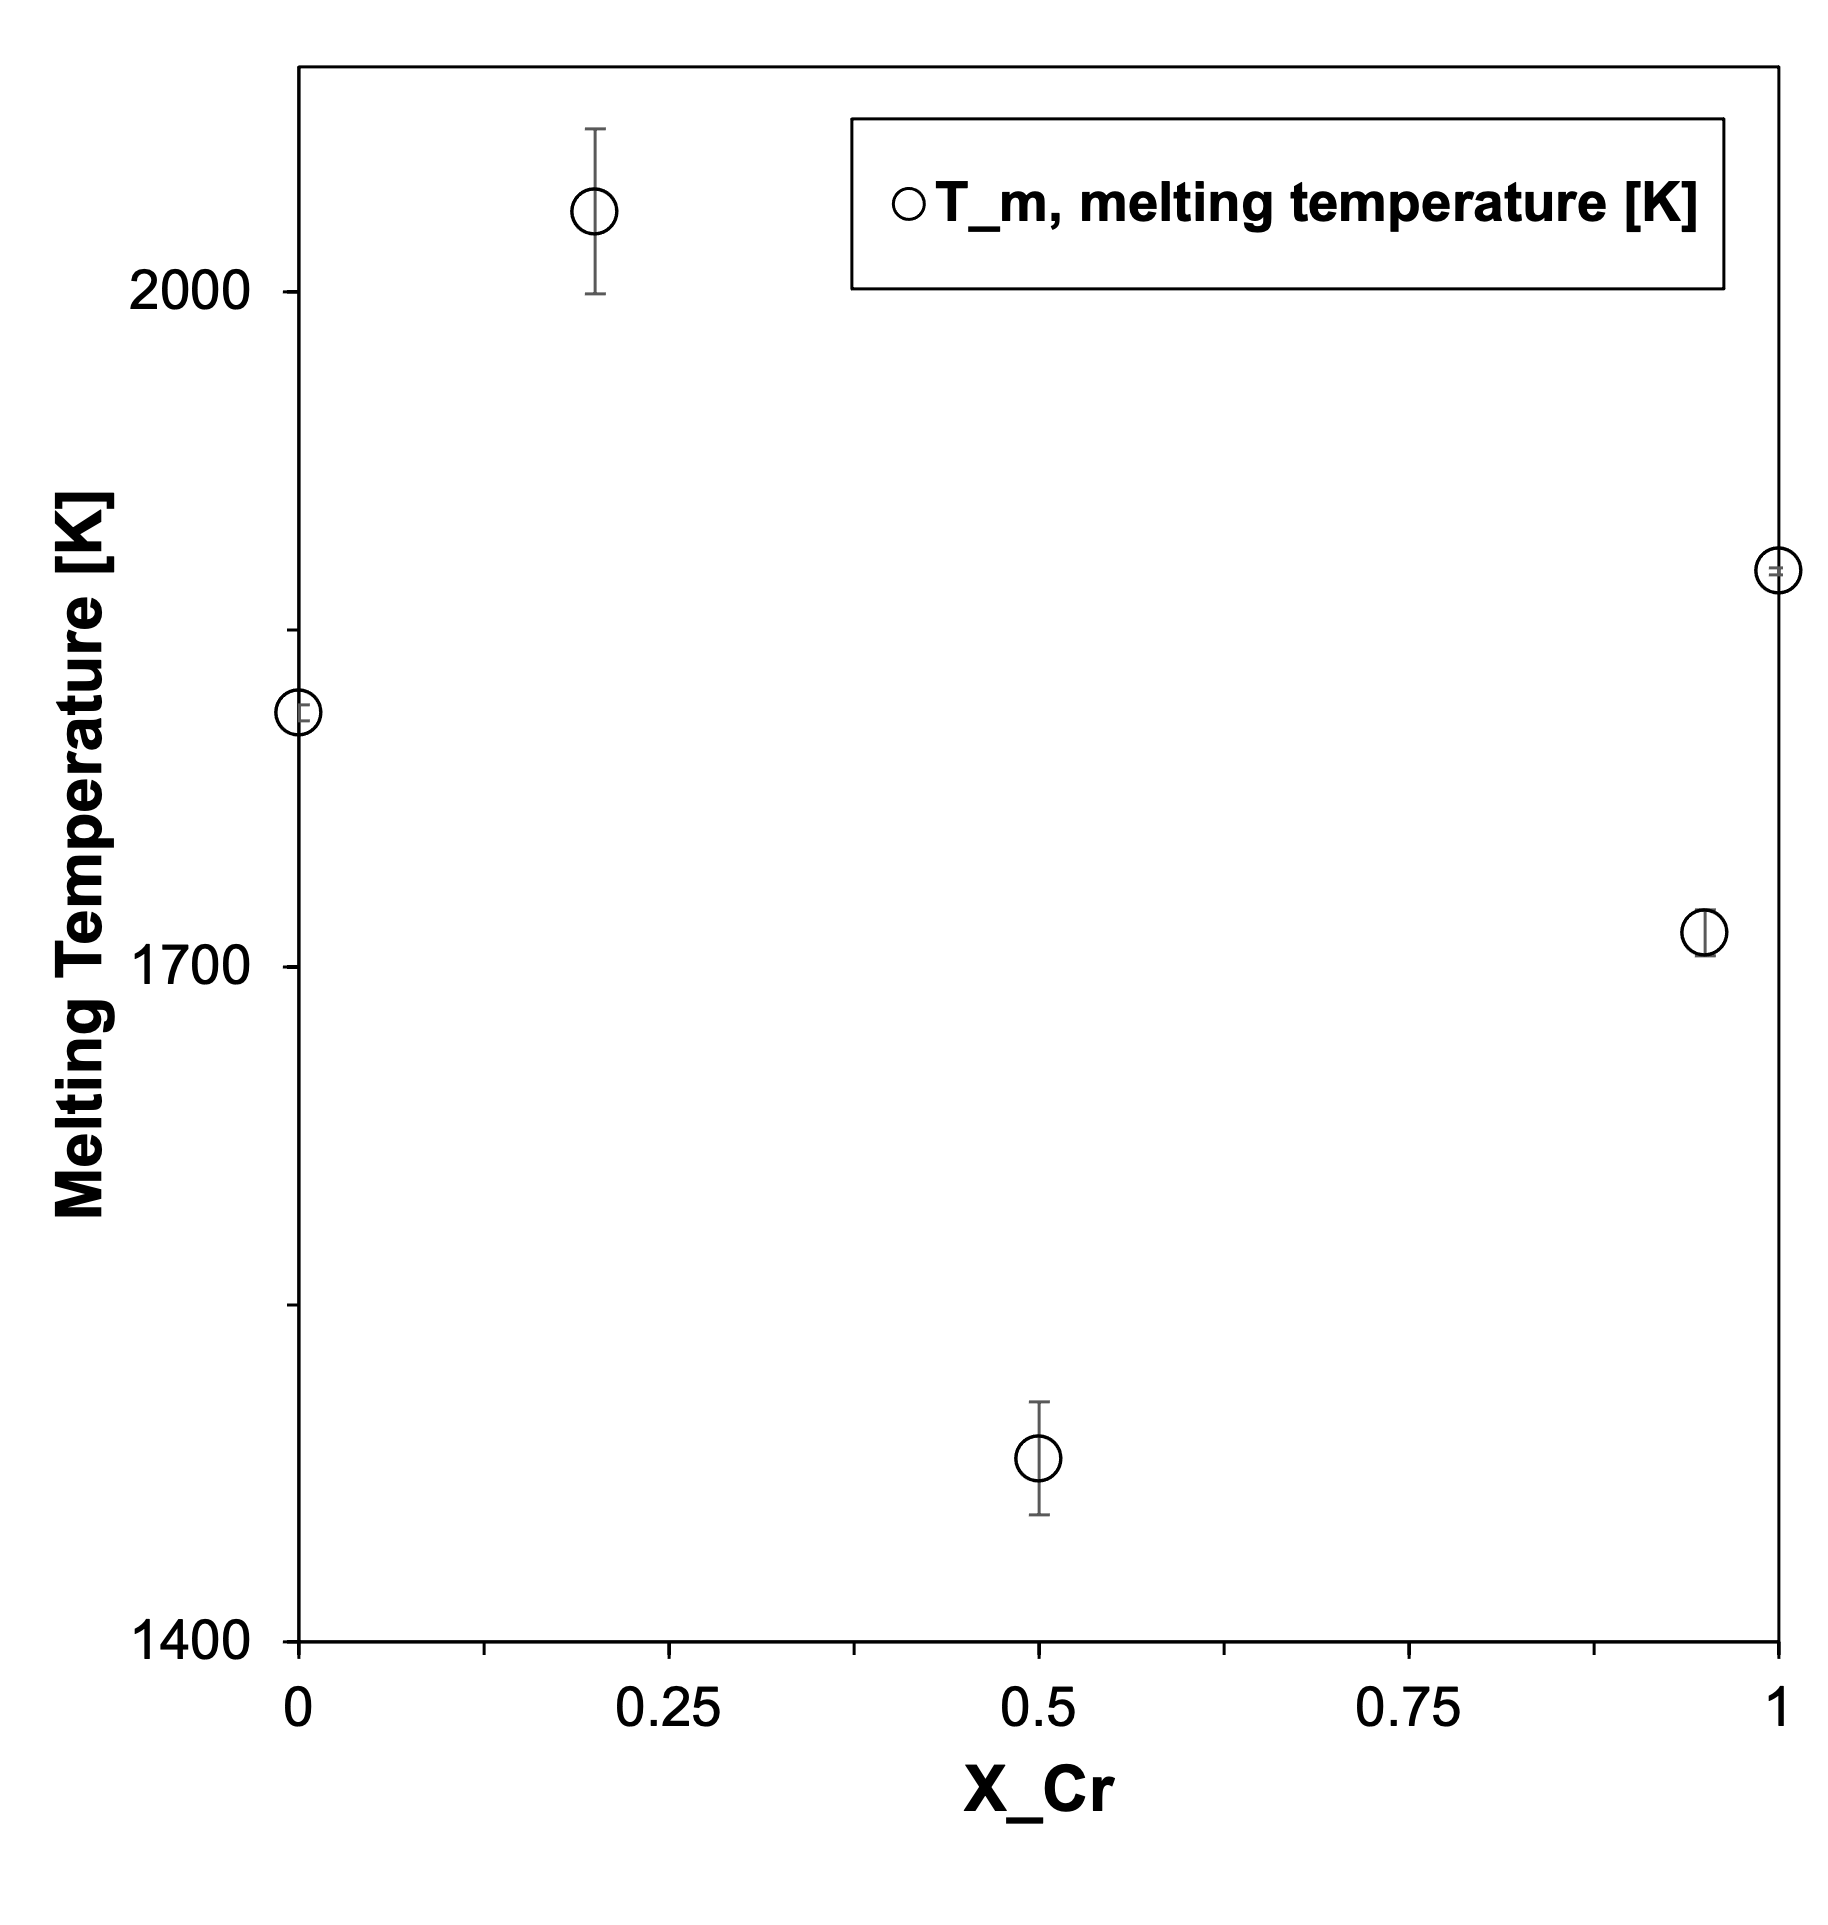
\includegraphics[width=\linewidth]{Parts/Figures/TMvsX_v2.png}
         \caption{\(T_M\), melting temperature, indicating how the thermal stability of the material changes with Cr composition.}
         \label{fig3b}
     \end{subfigure}
     \begin{subfigure}{0.3\textwidth}
         \centering
         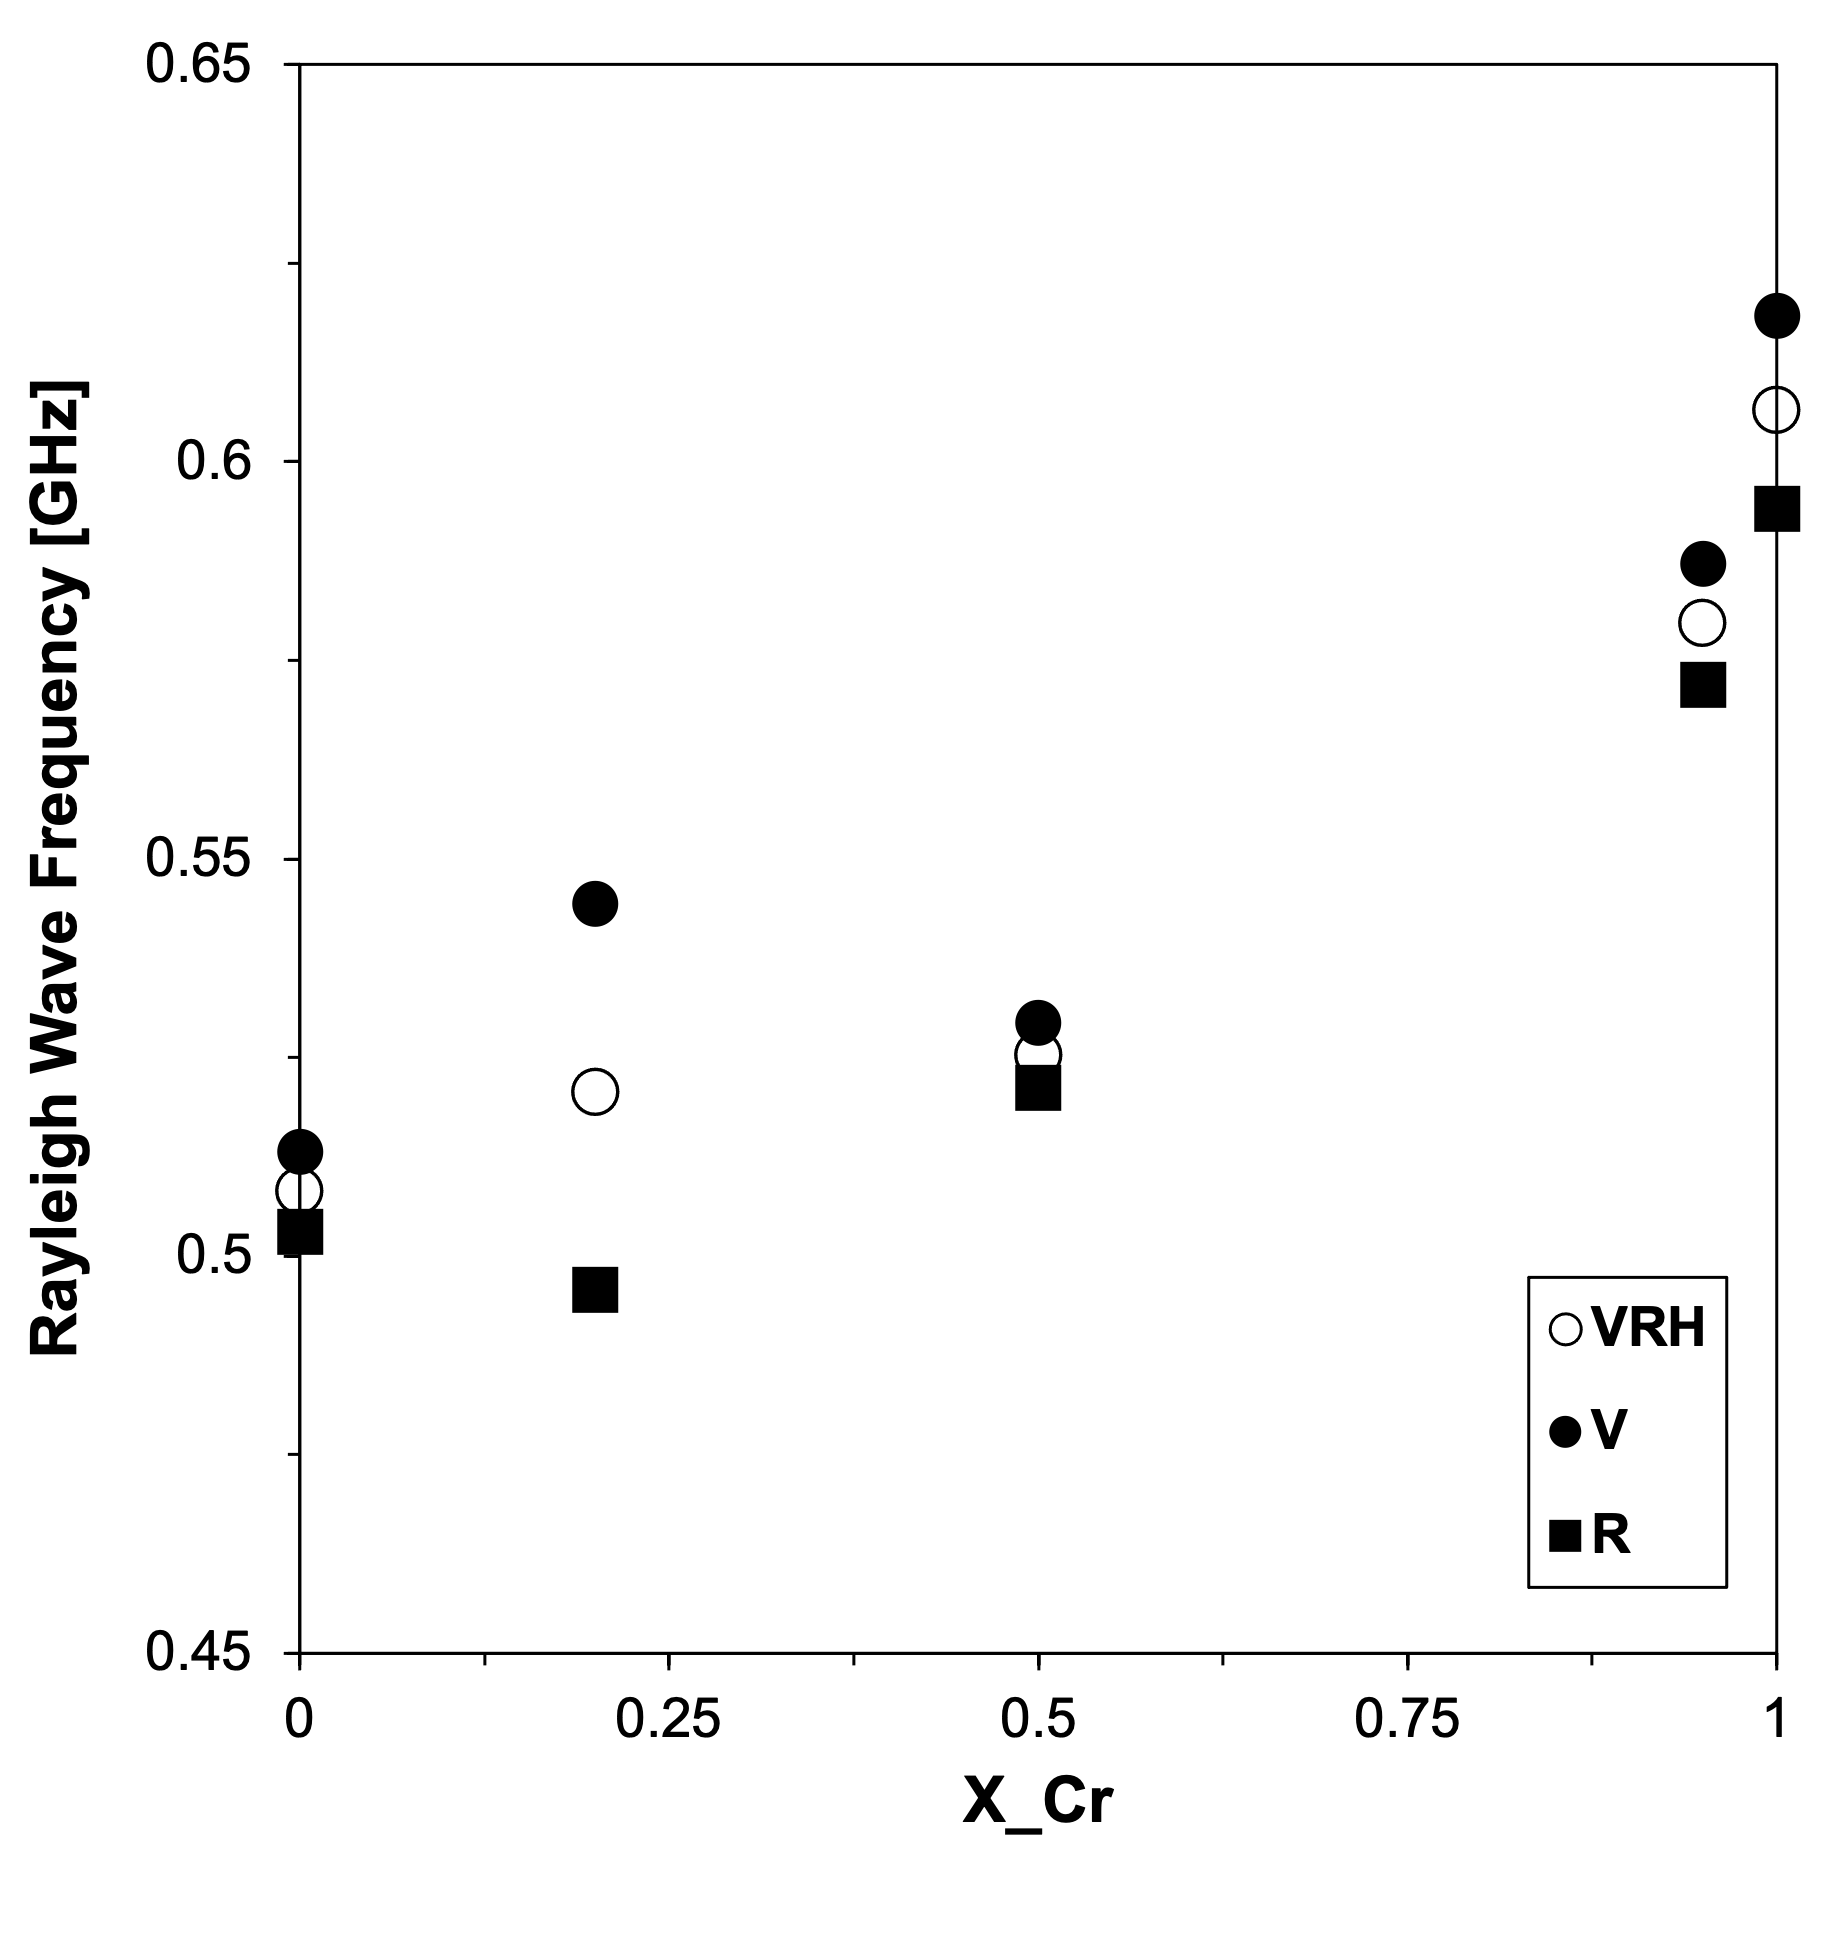
\includegraphics[width=\linewidth]{Parts/Figures/f_rwVsX_vF.png}
         \caption{Rayleigh wave frequencies, illustrating the impact of spinodal decomposition on the material's surface acoustic properties.}
         \label{fig3c}
     \end{subfigure}
     \begin{subfigure}{0.3\textwidth}
         \centering
         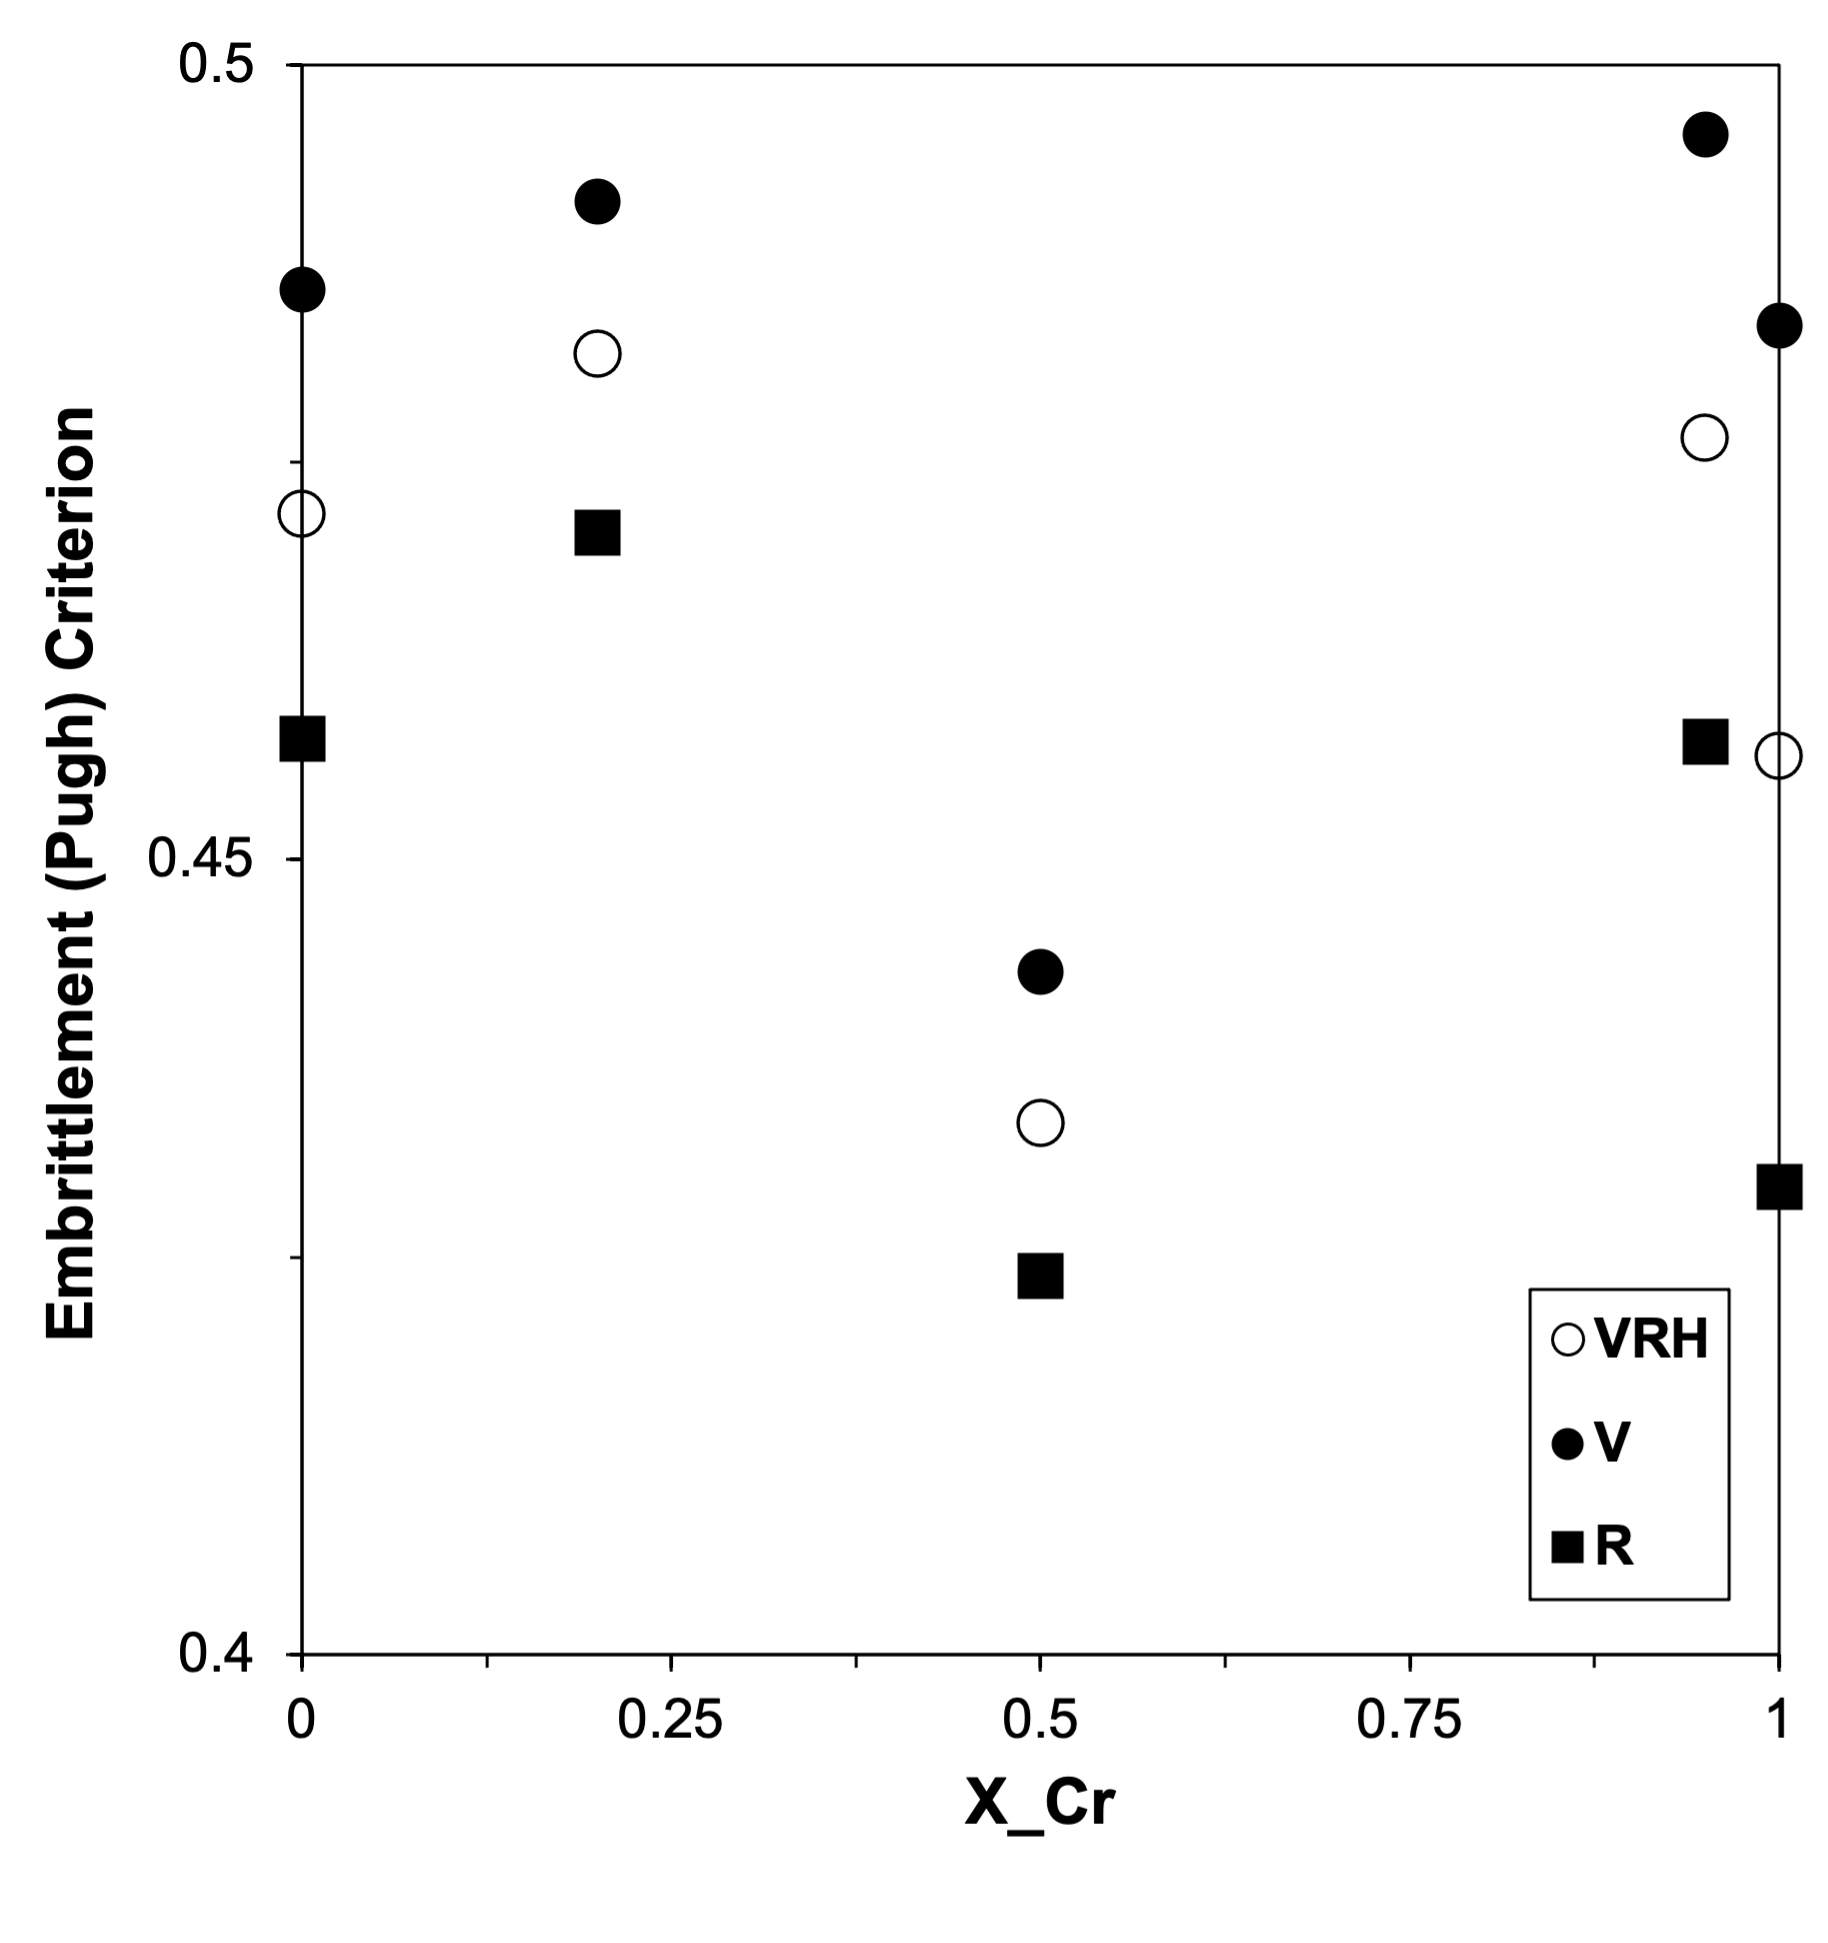
\includegraphics[width=\linewidth]{Parts/Figures/EvsX_vF.png}
         \caption{Embrittlement (Pugh) Criterion, calculated to evaluate the embrittlement risk associated with varying Cr compositions.}
         \label{fig3d}
     \end{subfigure}
	\caption{(a) The enthalpy of mixing demonstrates the thermodynamic drive towards phase separation indicative of spinodal decomposition, affecting the material's mechanical integrity. (b) Variations in the melting temperature as a function of Cr composition offer insights into the thermal stability and potential phase transformations within the alloy. (c) Changes in Rayleigh wave frequencies across compositions highlight alterations in surface acoustic properties, correlating with mechanical behavior. (d) The Embrittlement (Pugh) Criterion allows for assessing the risk of material embrittlement due to changes in composition, crucial for ensuring material reliability in critical applications.}
	\label{fig3}
\end{sidewaysfigure}


\begin{sidewaysfigure}[!ht]
    \centering
    \begin{subfigure}{0.9\textwidth}
        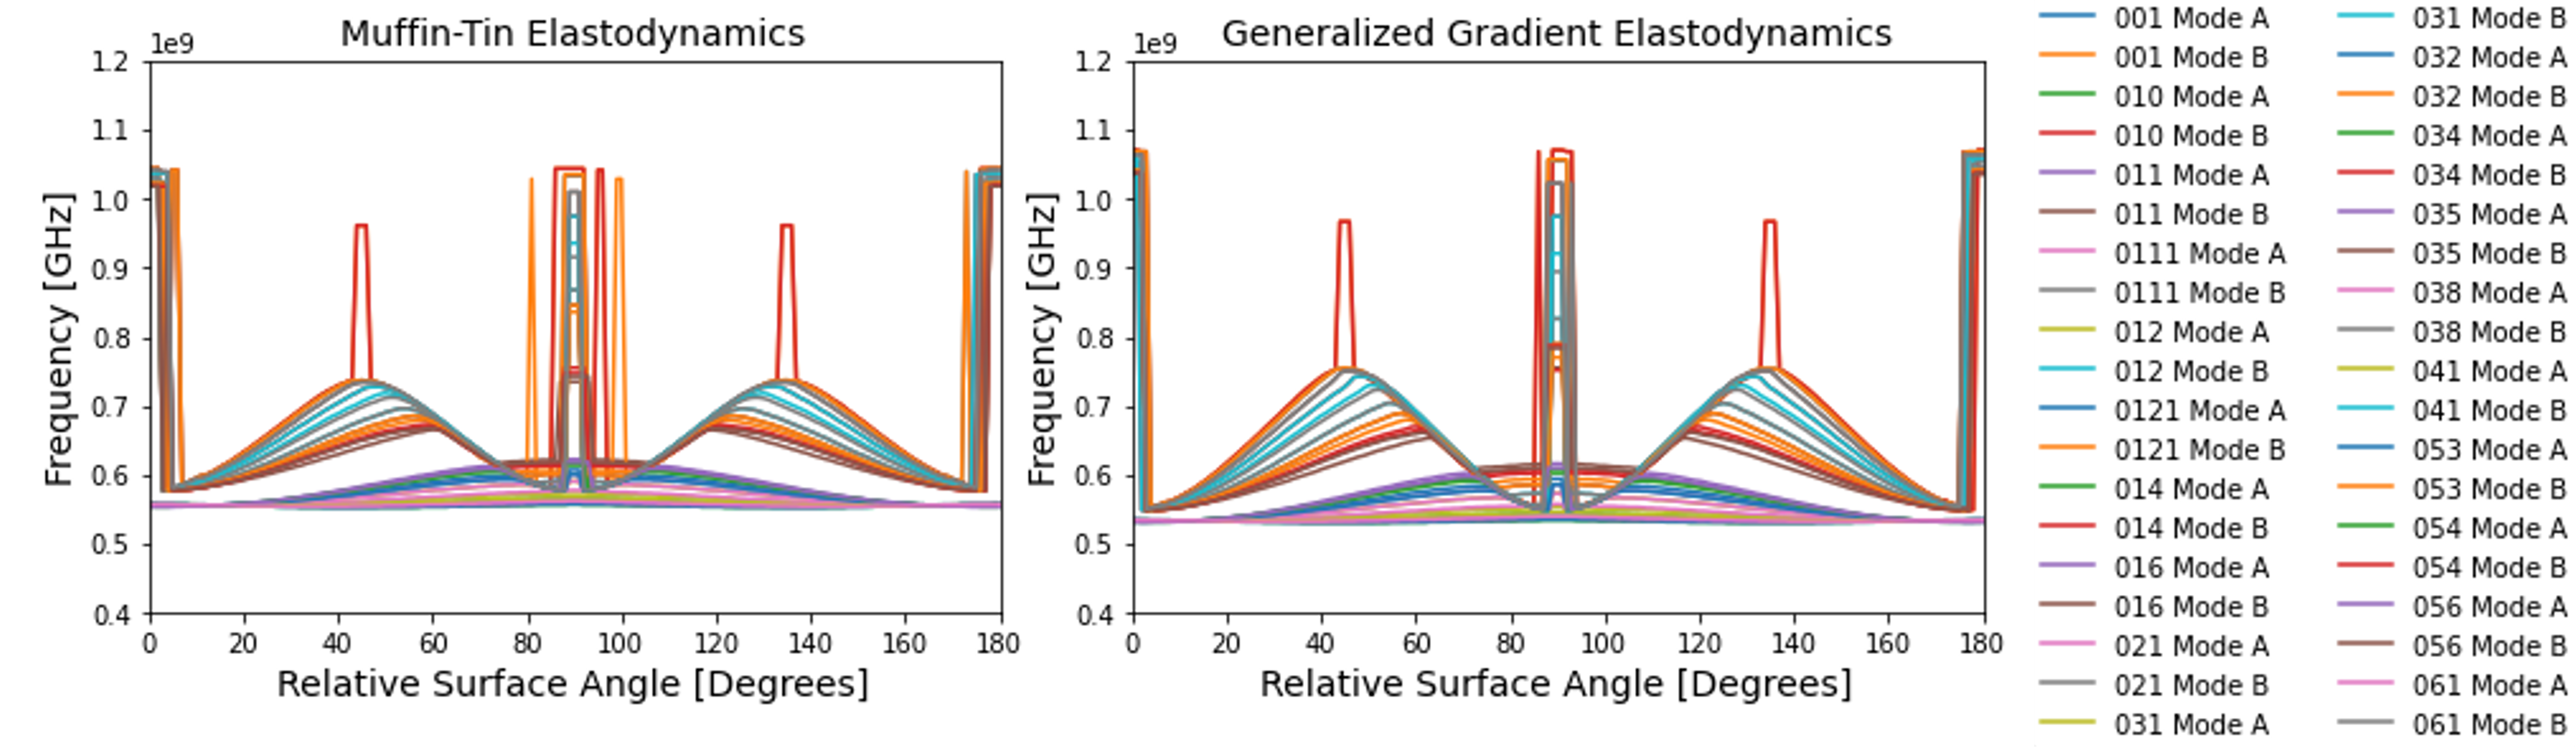
\includegraphics[width=\textwidth]{Parts/Figures/smoking-gun-v2.png}
        \caption{Predicted elastic frequencies showcasing the emergence of new modes within the elastodynamically-unallowed regions, signifying alterations in the material's mechanical properties due to spinodal decomposition.}
        \label{fig4a}
    \end{subfigure}
    \begin{subfigure}{0.35\textwidth}
        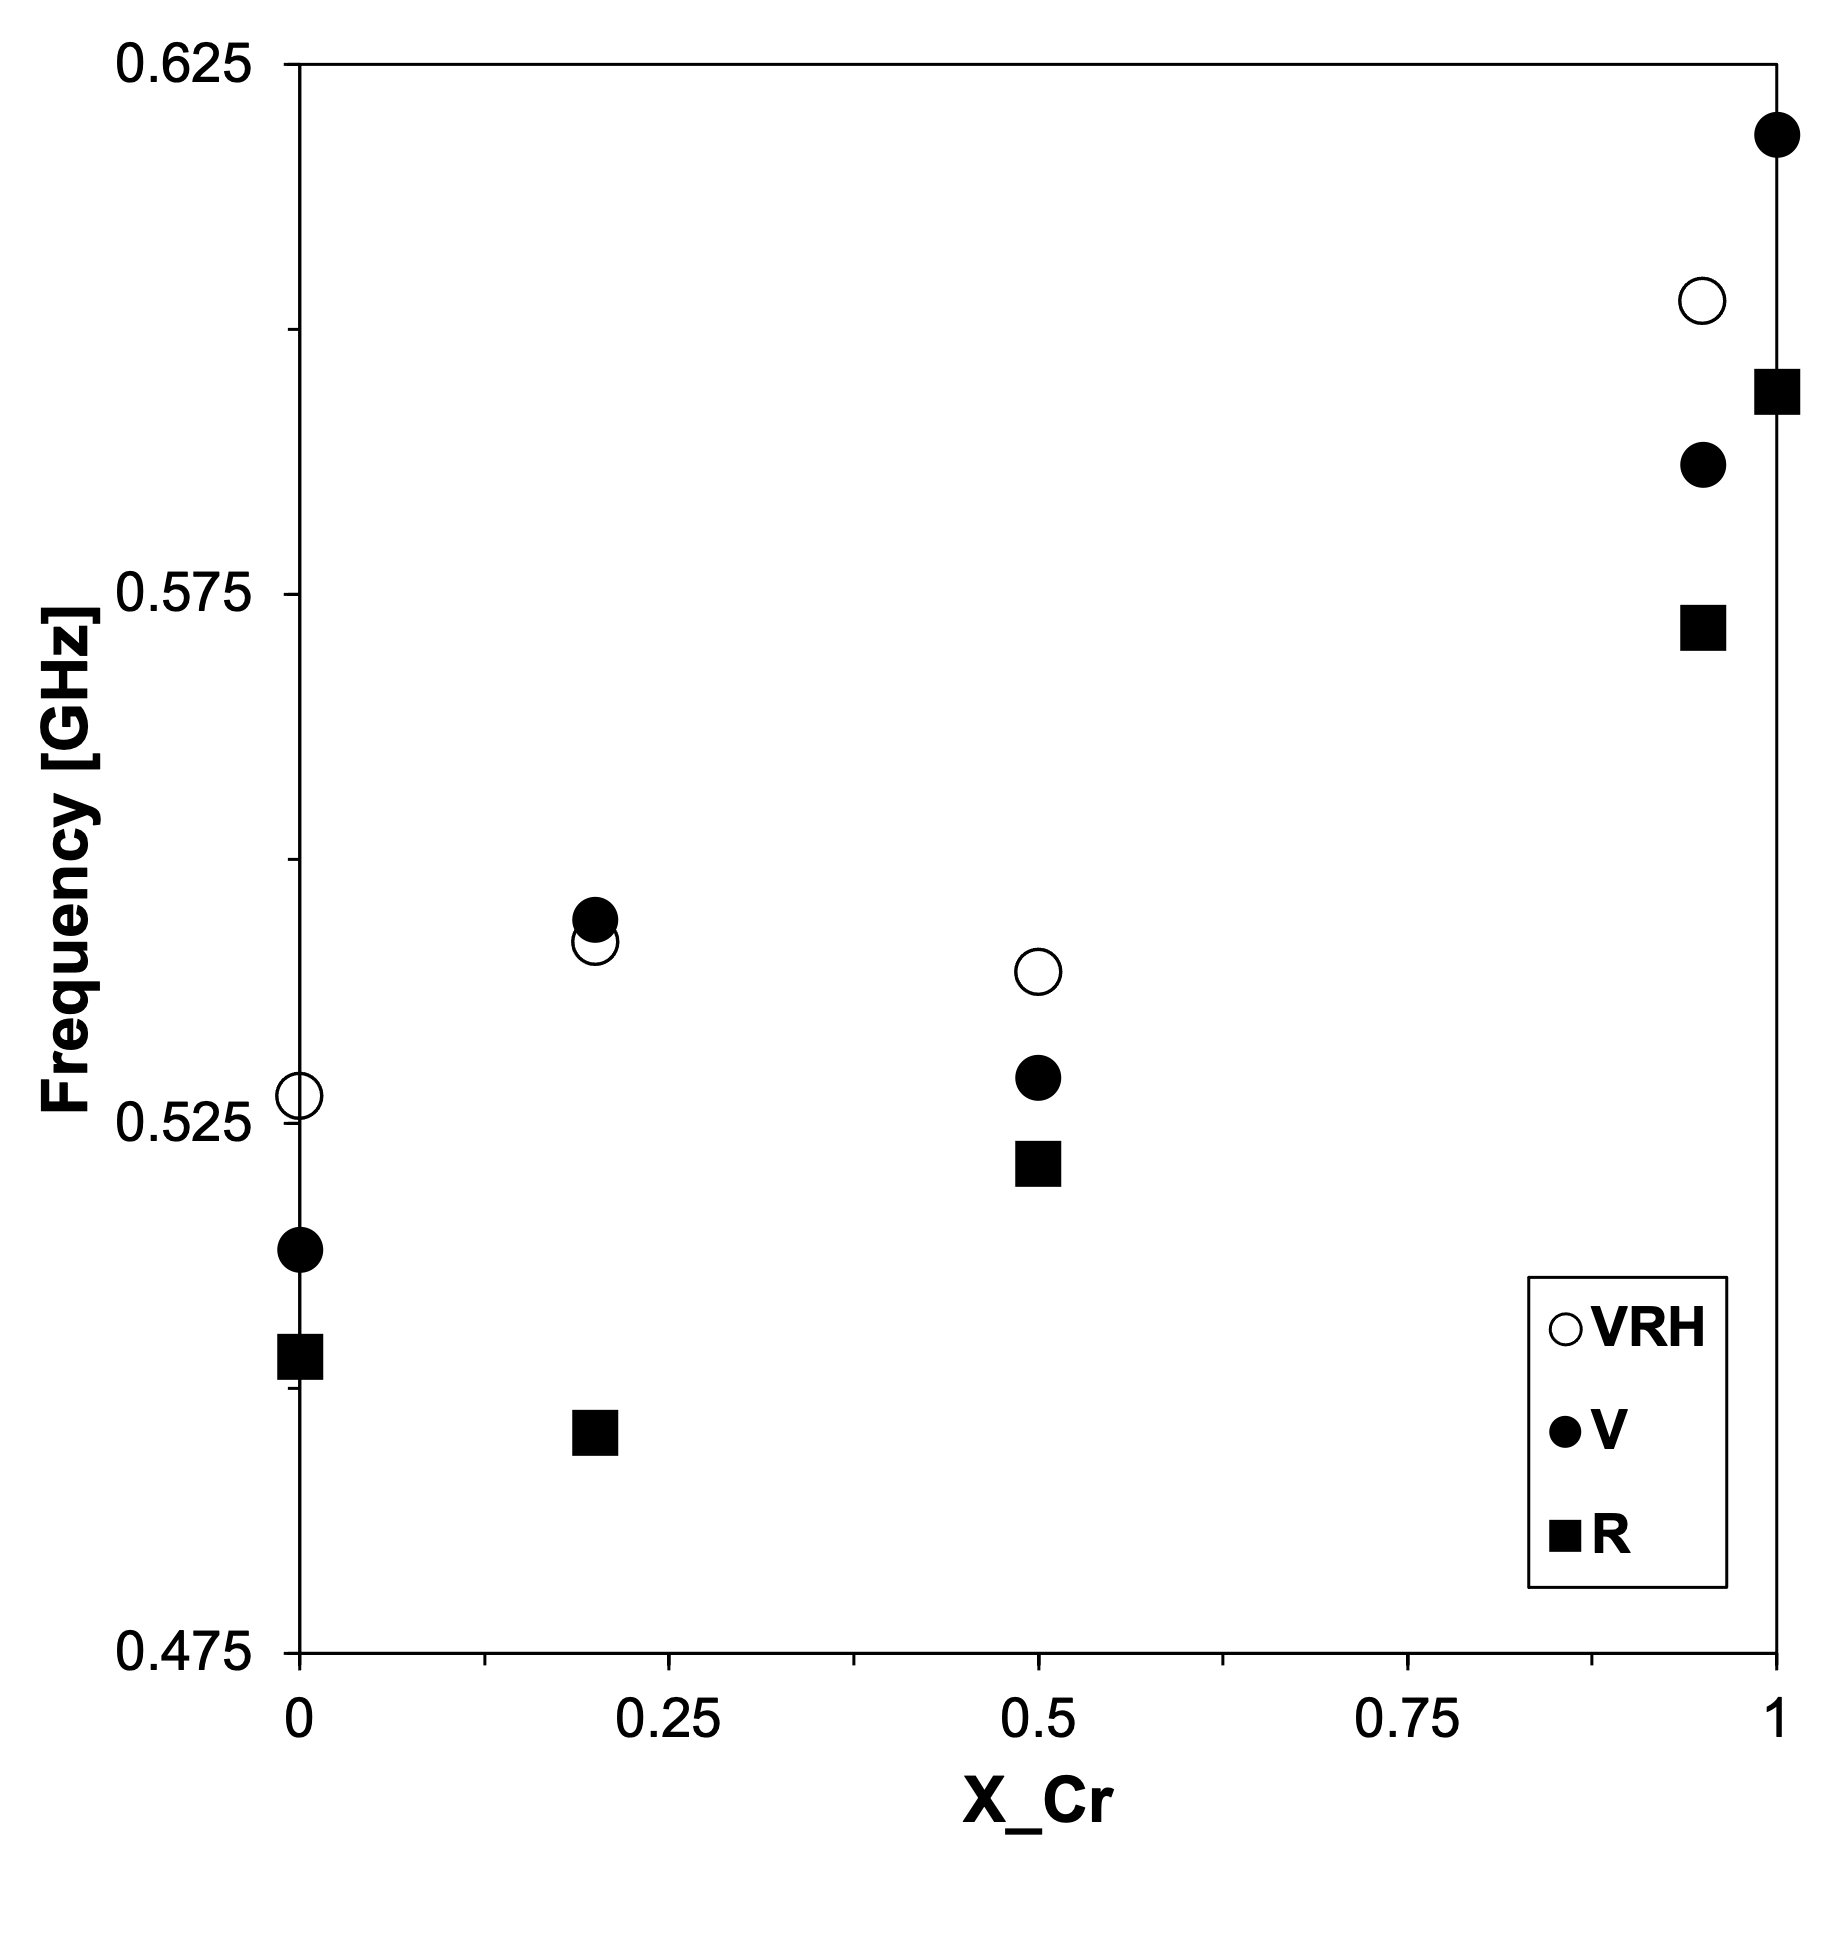
\includegraphics[width=\textwidth]{Parts/Figures/fvsX_v3.png}
        \caption{Calculated acoustic frequencies across different Cr compositions, illustrating the material's acoustic response variability with composition. This graph provides a quantitative measure of the material's mechanical behavior and its dependence on the microstructural characteristics induced by varying chromium content.}
        \label{fig4b}
    \end{subfigure}
    \begin{subfigure}{0.5\textwidth}
        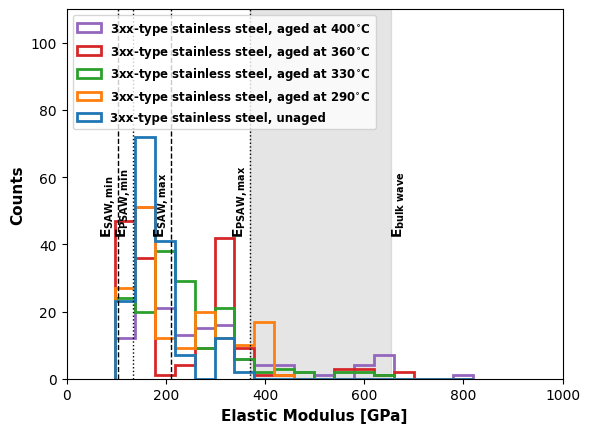
\includegraphics[width=\textwidth]{Parts/Figures/experimental-moduli-hist.png}
        \caption{Measured elastic moduli distribution from experimental data, highlighting the range and variability of material properties within stainless steel samples subjected to different thermal aging processes. The distribution underscores the significant impact of microstructural changes, such as spinodal decomposition, on the material's overall stiffness and mechanical integrity.}
        \label{fig4c}
    \end{subfigure}
    \caption{(a) Quantum elastodynamic frequencies obtained from density functional theory calculations reveal the complex interplay between microstructural evolution and mechanical properties in stainless steels undergoing spinodal decomposition. These findings are corroborated by (b) calculated acoustic frequencies that vary with Cr composition, providing a link between composition, microstructure, and acoustic properties. (c) The distribution of measured elastic moduli further validates the theoretical predictions, illustrating the broad impact of aging and compositional changes on the material's mechanical performance.}
    \label{fig4}
\end{sidewaysfigure}


\begin{sidewaysfigure}[!ht]
	\centering
	\begin{subfigure}{0.3\textwidth}
         \centering
         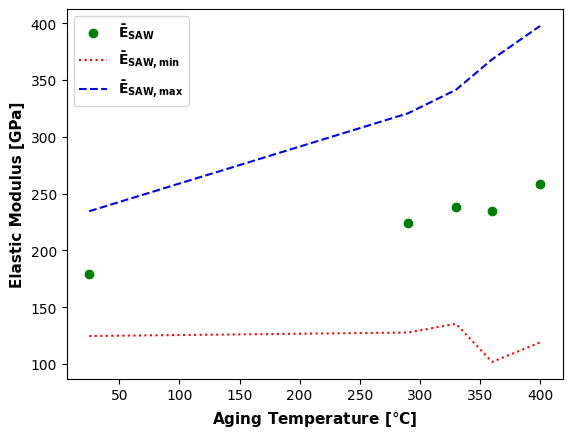
\includegraphics[width=\linewidth]{Parts/Figures/experimental-moduli-trend.png}
         \caption{Experimental elastic moduli of aged steels, displaying how aging temperature influences the material's stiffness. This graph illustrates the correlation between thermal treatment and the increase in elastic moduli, indicative of the material's response to microstructural changes over time.}
         \label{fig5a}
     \end{subfigure}
     \hfill
     \begin{subfigure}{0.3\textwidth}
         \centering
         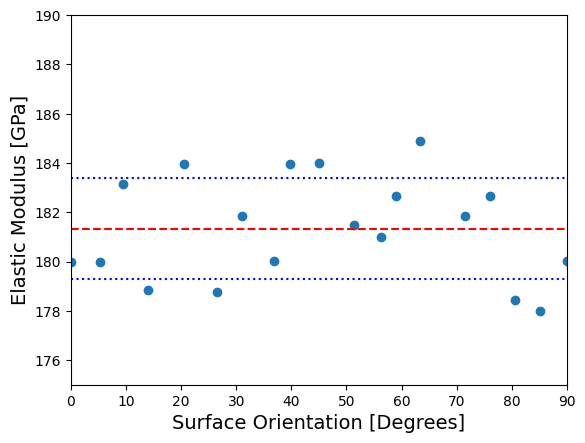
\includegraphics[width=\linewidth]{Parts/Figures/approximate-elastic-moduli-from-SAW-measurements-pristine.png}
         \caption{Theoretical elastic moduli of pristine steels, offering a baseline comparison for understanding how spinodal decomposition affects material properties before and after aging. This comparison elucidates the stiffening effect of microstructural evolution on the alloy's mechanical behavior.}
         \label{fig5b}
     \end{subfigure}
     \hfill
     \begin{subfigure}{0.3\textwidth}
         \centering
         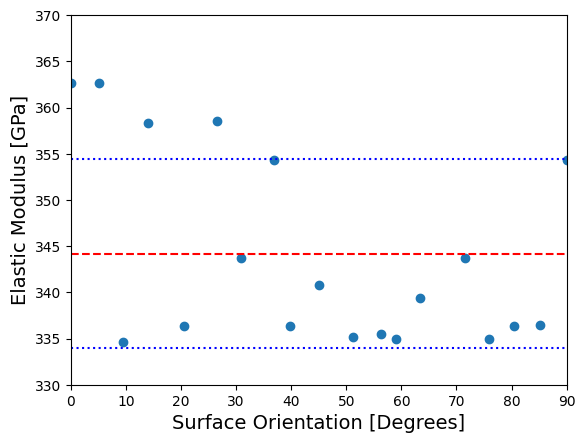
\includegraphics[width=\linewidth]{Parts/Figures/approximate-elastic-moduli-from-SAW-measurements-spindec.png}
         \caption{Theoretical elastic moduli of spinodally decomposed steels, demonstrating the pronounced impact of microstructural evolution on the alloy's stiffness. This direct comparison to pristine conditions highlights the significant role of chromium composition and thermal aging in material performance.}
         \label{fig5c}
     \end{subfigure}
     \hfill
     \begin{subfigure}{0.3\textwidth}
         \centering
         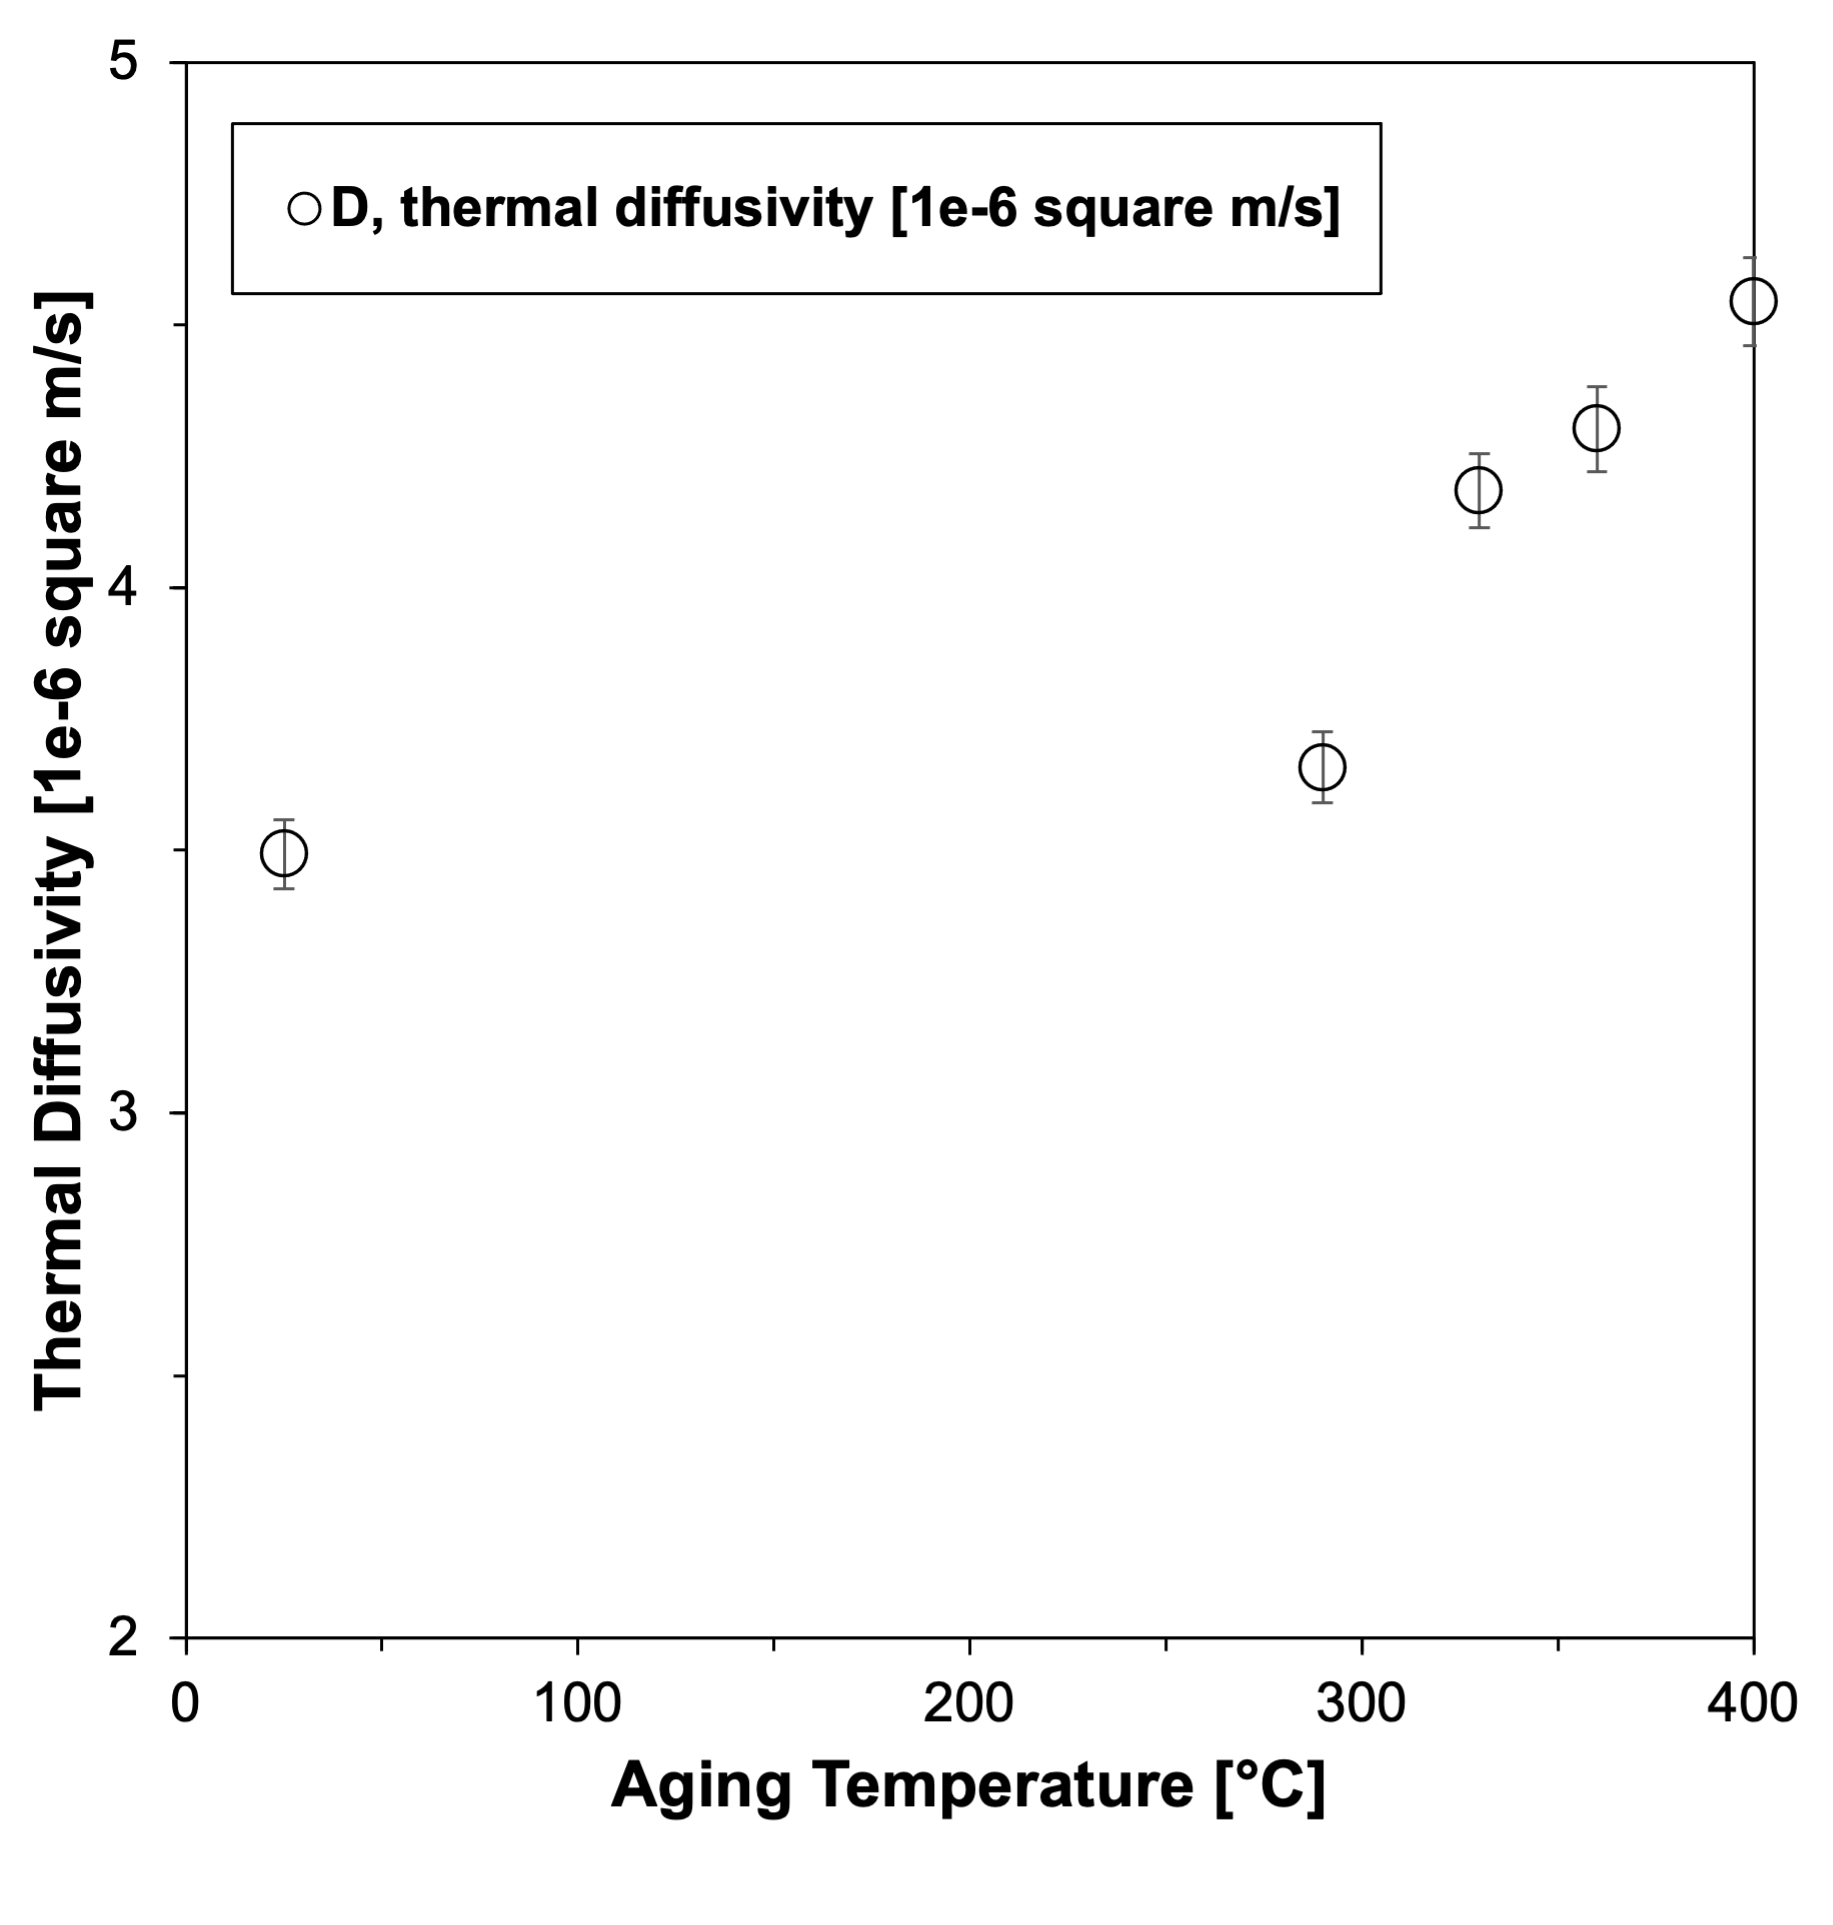
\includegraphics[width=\linewidth]{Parts/Figures/DvsT_CF8_30khrs_v2.png}
         \caption{\(D^{exp}_{thermal}\), experimental thermal diffusivity as measured in aged stainless steel, illustrating the thermal transport characteristics and their variation with temperature. This metric provides insights into the thermal stability and heat dissipation capabilities of the material post-aging.}
         \label{fig5d}
     \end{subfigure}
     \hfill
     \begin{subfigure}{0.3\textwidth}
         \centering
         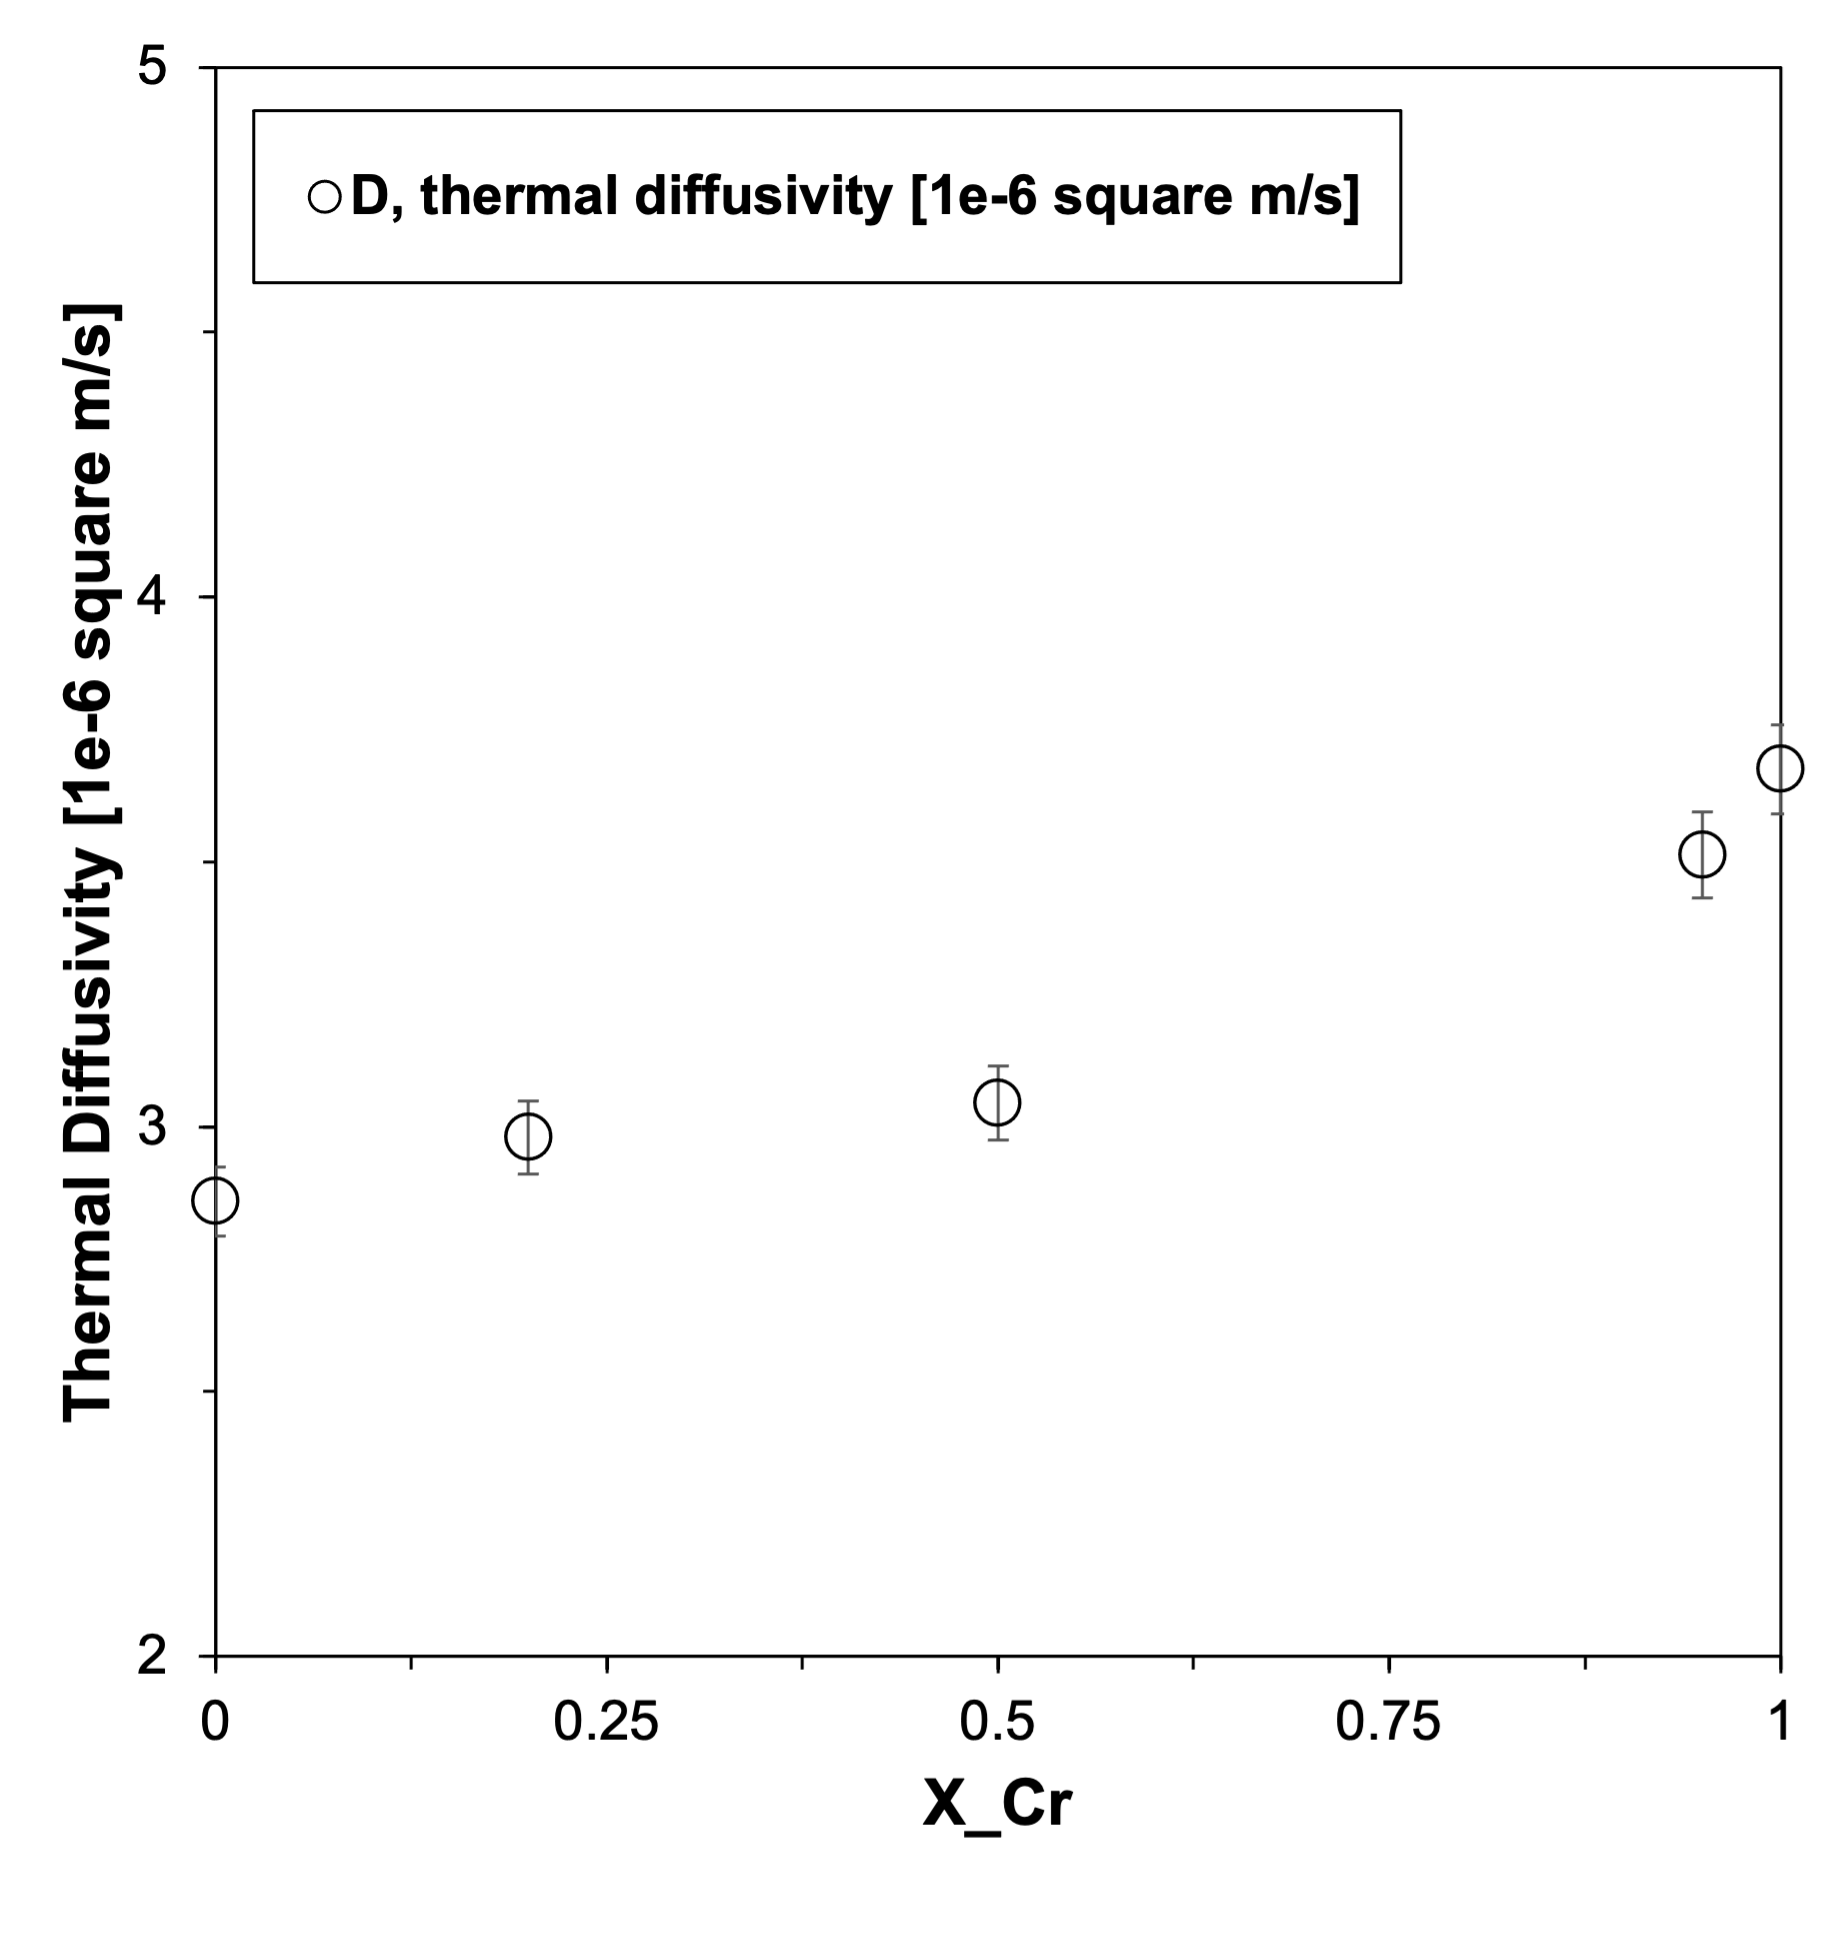
\includegraphics[width=\linewidth]{Parts/Figures/DvsX_v4.png}
         \caption{\(D^{theoretical}_{thermal}\), theoretical thermal diffusivity indicating the expected thermal behavior based on composition and microstructural considerations. This predictive analysis aids in understanding the thermal management potential of the alloy across a range of compositions.}
         \label{fig5e}
     \end{subfigure}
     \hfill
     \begin{subfigure}{0.3\textwidth}
         \centering
         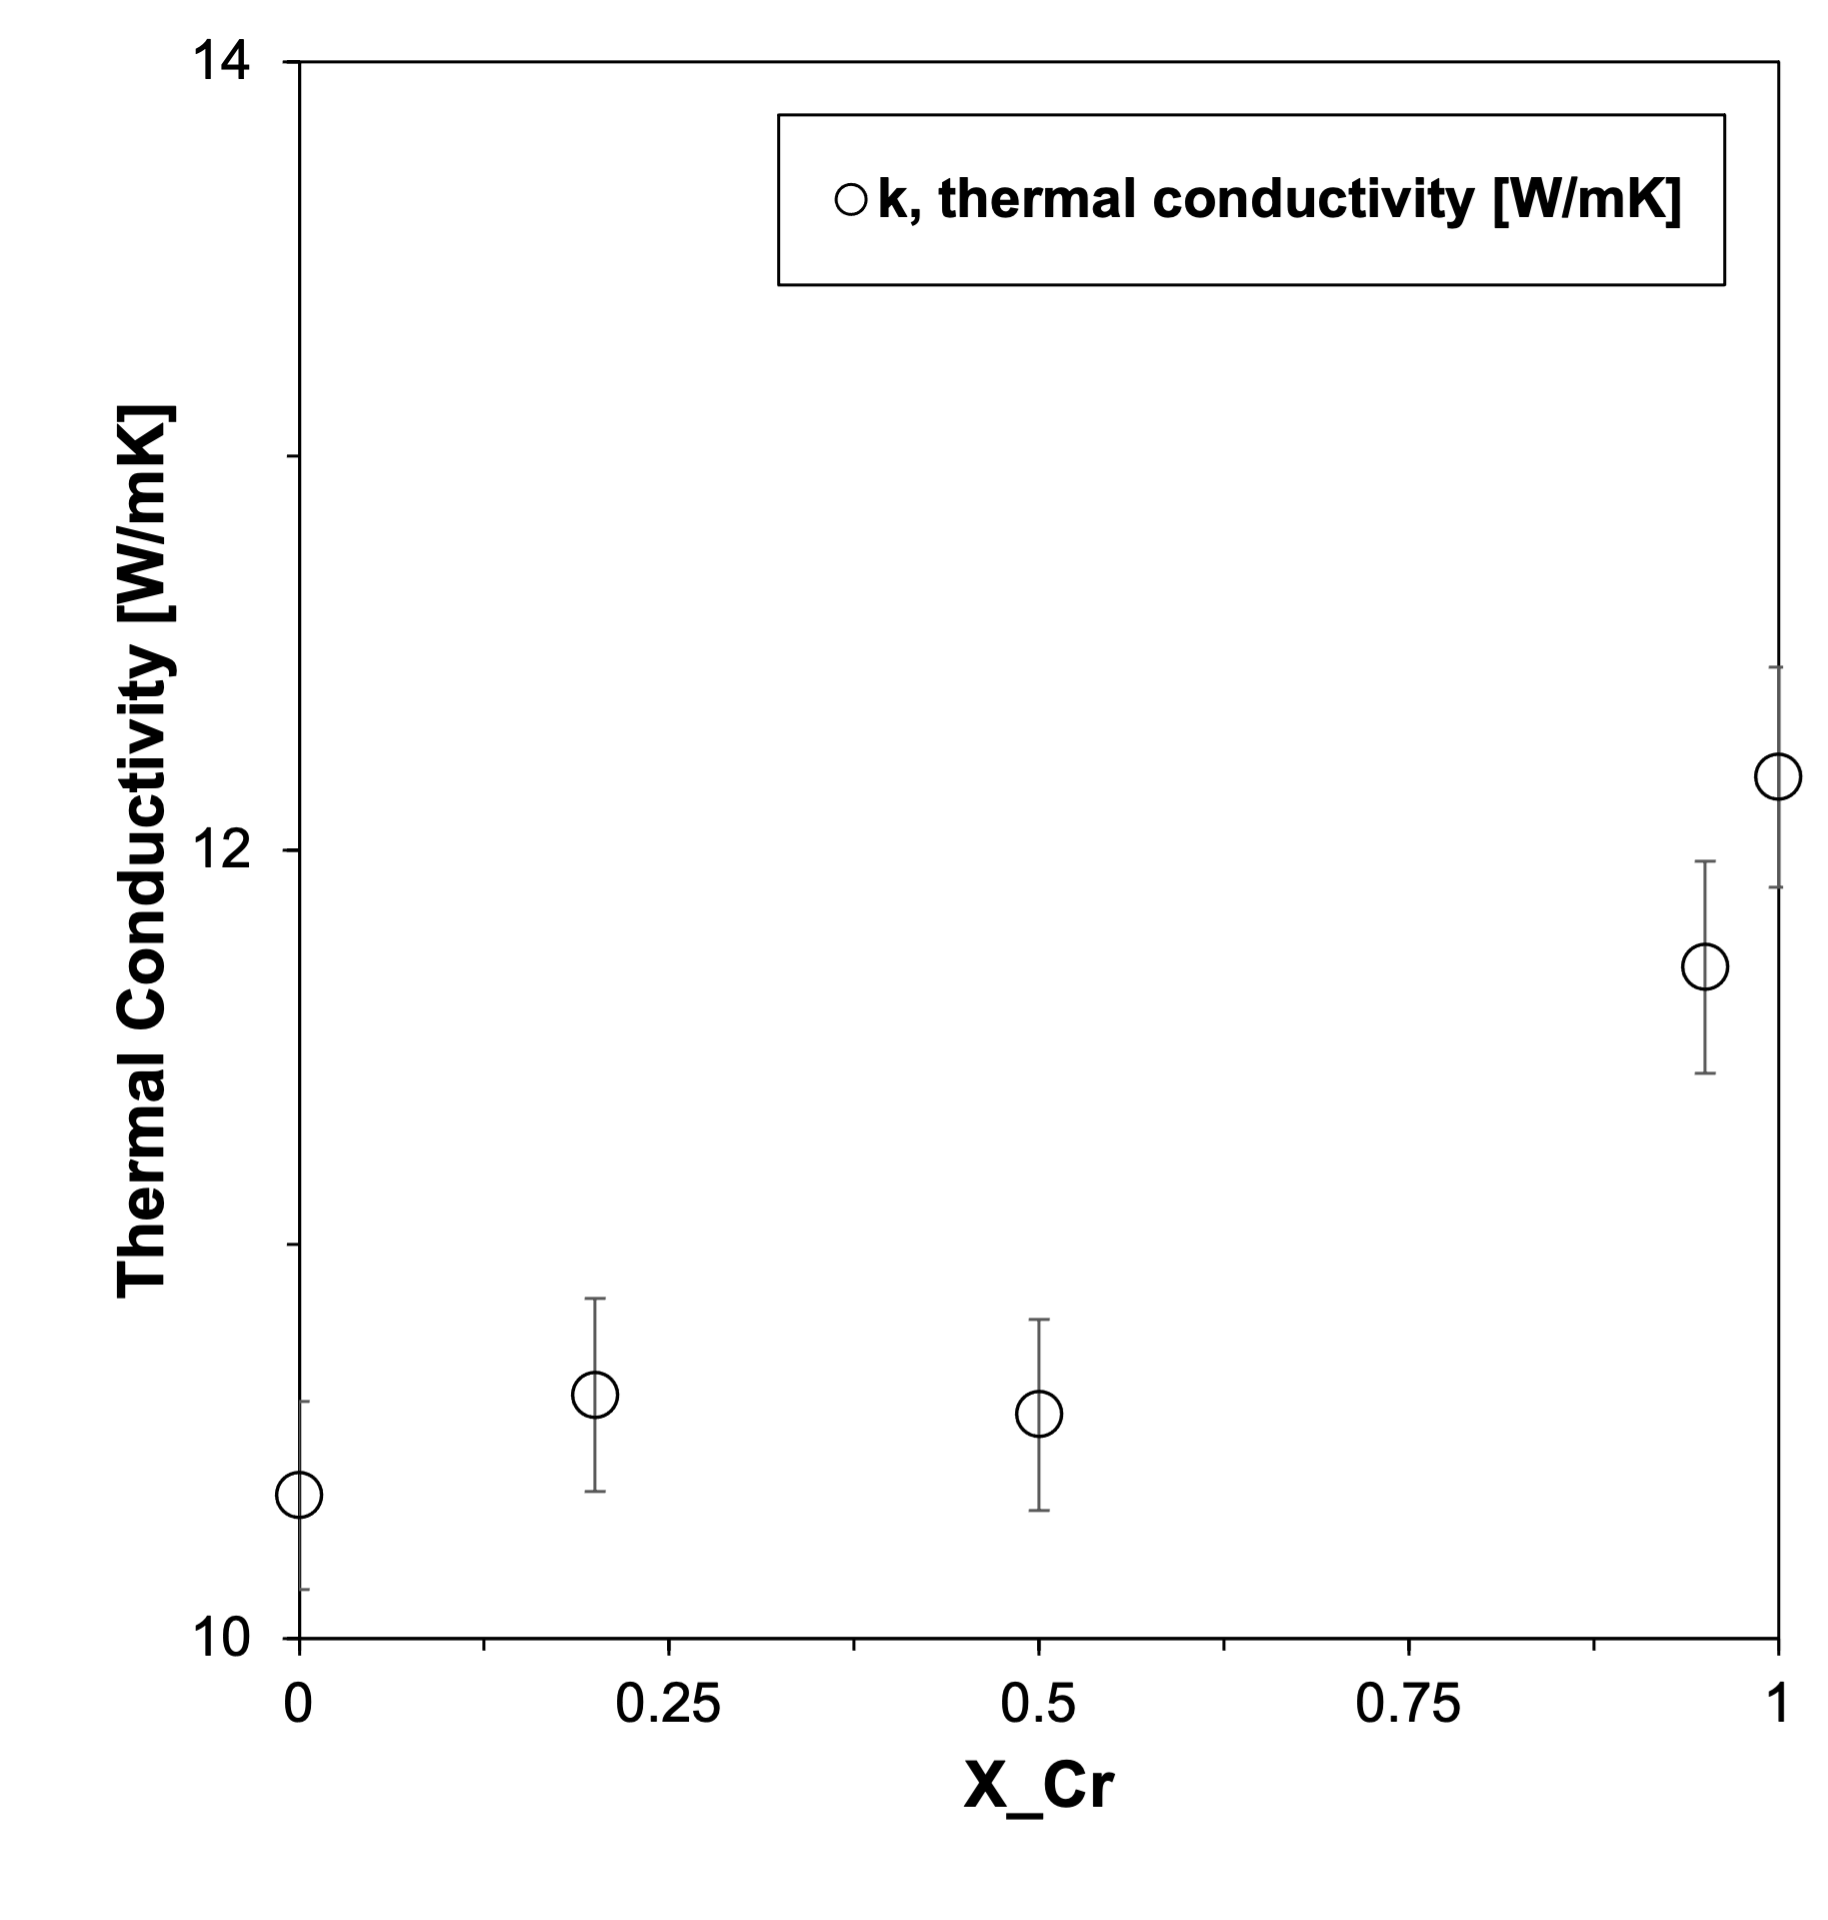
\includegraphics[width=\linewidth]{Parts/Figures/KvsX_v2.png}
         \caption{\(\kappa^{theoretical}_{thermal}\), thermal conductivity, showcasing the theoretical prediction of how efficiently the material conducts heat. This property is crucial for applications where thermal management is key, and it is influenced by the alloy's microstructure and composition.}
         \label{fig5f}
     \end{subfigure}
	\caption{Comprehensive analysis combining experimental and theoretical insights into the thermal and mechanical properties of stainless steels subjected to thermal aging. (a) Experimental elastic moduli trends with aging temperature highlight the stiffening effect of microstructural evolution. (b) and (c) Theoretical predictions for pristine and spinodally decomposed steels provide a comparative framework for assessing the impact of spinodal decomposition on material properties. (d) Experimental thermal diffusivity measurements, alongside (e) theoretical predictions for thermal diffusivity and (f) thermal conductivity, offer a holistic view of the material's thermal and mechanical behavior post-aging, emphasizing the interconnectedness of thermal properties, mechanical performance, and microstructural characteristics.}
	\label{fig5}
\end{sidewaysfigure}


\end{document}
